% =====================================================================
%  ВКР бакалавра. Тема: «Исследование методов обработки данных в
%  фазочувствительной рефлектометрии на длинных оптических линиях
%  с усилителями».
%  Оформление - строго по Приложению 2 к Положению о ВКР МФТИ.
% =====================================================================

\documentclass[12pt,a4paper]{extarticle}

% - Кодировка, языки, шрифты ---------
\usepackage{fontspec}
\setmainfont{Times New Roman}
\setmonofont{Courier New}
\usepackage{polyglossia}
\setdefaultlanguage{russian}
\setotherlanguage{english}
\newfontfamily\cyrillicfont{Times New Roman}[Script=Cyrillic]
\newfontfamily\cyrillicfonttt{Courier New}[Script=Cyrillic]

% - Поля строго по Приложению 2 ---------
% левое 30 мм, правое 15 мм, верхнее 20 мм, нижнее 20 мм.
\usepackage[a4paper, left=30mm, right=15mm, top=20mm, bottom=20mm]{geometry}

% - Абзацный отступ 1.25 см, интервал 1.5, абзацный отступ - у каждого
%     первого абзаца раздела ---------
\usepackage{indentfirst}
\setlength{\parindent}{1.25cm}
\linespread{1.5}
\setlength{\parskip}{0pt}

% Выравнивание основного текста по ширине поля - это поведение по умолчанию.
% Чтобы избежать переполнений строки на сложно-перебиваемых русско-английских
% терминах, расслабляем критерии разбиения абзаца.
\emergencystretch=2.5em
\tolerance=1500
\hyphenpenalty=100

% - Математика, графика, таблицы --------
\usepackage{amsmath, amssymb, amsfonts}
\usepackage{graphicx}
\graphicspath{{figures/}{../slides/assets/}{../reports/figures/}{../images/}}
\usepackage{booktabs}
\usepackage{array}
\usepackage{makecell}
\usepackage{caption}
% Подписи рисунков остаются по центру; подписи таблиц - слева через дефис
% (по Положению МФТИ Прил. 2: «Наименование таблицы помещать над таблицей
% слева, без абзацного отступа в одну строку с её номером через тире»).
\DeclareCaptionLabelSeparator{hyphen}{ - }
% Подписи рисунков и таблиц - 12 пт (normalsize при documentclass 12pt),
% соответствует требованию Положения «подписи к рисункам, таблицам - 12 или 14 пт».
\captionsetup{font=normalsize, labelfont={normalsize,bf}, labelsep=endash, justification=centering}
\captionsetup[table]{font=normalsize, labelfont={normalsize,bf}, labelsep=hyphen,
  justification=raggedright, singlelinecheck=false}

% - Заголовки -----------
% Все заголовки 14 пт по Положению МФТИ. Визуальная иерархия:
% главы - 14 пт полужирные ПРОПИСНЫЕ; параграфы - 14 пт полужирные обычным
% регистром; подпараграфы - 14 пт курсив обычным регистром. Все центрированы.
\usepackage{titlesec}
\titleformat{\section}[block]
  {\normalfont\fontsize{14}{17}\bfseries\filcenter\MakeUppercase}
  {\thesection}{1em}{}
\titleformat{\subsection}[block]
  {\normalfont\fontsize{14}{17}\bfseries\filcenter}
  {\thesubsection}{1em}{}
\titleformat{\subsubsection}[block]
  {\normalfont\fontsize{14}{17}\itshape\filcenter}
  {\thesubsubsection}{1em}{}
\titlespacing*{\section}{0pt}{22pt}{14pt}
\titlespacing*{\subsection}{0pt}{14pt}{8pt}
\titlespacing*{\subsubsection}{0pt}{10pt}{6pt}

% - Содержание -----------
\usepackage{tocloft}
\renewcommand{\cfttoctitlefont}{\hfill\fontsize{14}{17}\bfseries}
\renewcommand{\cftaftertoctitle}{\hfill}
\setlength{\cftbeforesecskip}{4pt}

% - Колонтитулы и нумерация: внизу по центру, на «титульном» странице
%     номер не ставится. Поскольку титульный лист генерируется системой
%     МФТИ при загрузке файла, нумерация в нашем PDF начинается со страницы 2.
\usepackage{fancyhdr}
\pagestyle{fancy}
\fancyhf{}
\fancyfoot[C]{\thepage}
\renewcommand{\headrulewidth}{0pt}
\renewcommand{\footrulewidth}{0pt}

% - Прочее ------------
\usepackage{enumitem}
\setlist{itemsep=2pt, parsep=0pt, topsep=4pt}
\usepackage{microtype}
\usepackage{csquotes}
\usepackage[hidelinks]{hyperref}
\hypersetup{unicode=true, pdftitle={Исследование методов обработки данных в фазочувствительной рефлектометрии на длинных оптических линиях с усилителями}}

% - Сокращения для удобства ---------
\newcommand{\phiOTDR}{$\varphi$-OTDR}

% - Метаинформация ----------
\title{Исследование методов обработки данных в фазочувствительной\\ рефлектометрии на длинных оптических линиях с усилителями}

\begin{document}

% Титульный лист генерируется системой МФТИ при загрузке файла,
% поэтому в исходник он не входит. Нумерация - со страницы 2.
\setcounter{page}{2}

% =====================================================================
%  АННОТАЦИЯ (≤ 1500 знаков, без заголовка-номера)
% =====================================================================
\section*{Аннотация}
\addcontentsline{toc}{section}{Аннотация}

Работа посвящена разработке воспроизводимого алгоритма обработки данных фазочувствительной оптической рефлектометрии (\phiOTDR) на длинных волоконных линиях с распределёнными оптическими усилителями. Цель - автоматическая локализация возмущений вдоль волокна по данным когерентного обратного Рэлеевского рассеяния. Решены следующие задачи: (1)~из непрерывной записи аналого-цифрового преобразователя выделены отдельные рефлектограммы; (2)~устранён межтрассовый джиттер кросс-корреляционным выравниванием с критериями приёма; (3)~построен устойчивый к выбросам детектор, не зависящий от априорного знания частоты воздействия; (4)~метод валидирован на размеченном наборе из 130 файлов. Детектор сочетает медианный фон по времени, MAD-нормировку по дистанции и комбинированную спектральную оценку $S(g)$, агрегирующую пик и широкополосную энергию; пороговый отбор реализован двойным критерием. На размеченном наборе достигнуты F1\,=\,0{,}48, медианная ошибка локализации 61~м. Простой энергетический детектор-эталон даёт F1\,=\,0{,}33; это подтверждает необходимость спектральных признаков для устойчивой работы в условиях неоднородного по дистанции фона длинной линии.

\newpage

% =====================================================================
%  СОДЕРЖАНИЕ
% =====================================================================
\renewcommand{\contentsname}{\hfill Содержание \hfill}
\tableofcontents

\newpage

% =====================================================================
%  ОБОЗНАЧЕНИЯ И СОКРАЩЕНИЯ
% =====================================================================
\section*{Обозначения и сокращения}
\addcontentsline{toc}{section}{Обозначения и сокращения}

В работе используются следующие сокращения и условные обозначения.

\vspace{6pt}
\noindent
\begin{tabular}{@{}p{2.8cm} p{12.3cm}@{}}
АЦП & аналого-цифровой преобразователь \\
МД  & медианное абсолютное отклонение (см. MAD) \\
ASE & усиленная спонтанная эмиссия (Amplified Spontaneous Emission) \\
CWT & непрерывное вейвлет-преобразование (Continuous Wavelet Transform) \\
EDFA & эрбиевый волоконно-оптический усилитель (Erbium-Doped Fiber Amplifier) \\
FFT & быстрое преобразование Фурье (Fast Fourier Transform) \\
F1 & F1-мера, гармоническое среднее Precision и Recall \\
FP & ложное срабатывание (False Positive) \\
HMM & скрытые марковские модели (Hidden Markov Models) \\
MAD & медианное абсолютное отклонение (Median Absolute Deviation) \\
ML & машинное обучение (Machine Learning) \\
OTDR & оптическая рефлектометрия во временной области (Optical Time-Domain Reflectometry) \\
$\varphi$-OTDR & фазочувствительная OTDR (Phase-sensitive OTDR) \\
Precision & точность бинарного классификатора, $\mathrm{TP}/(\mathrm{TP}+\mathrm{FP})$ \\
Recall & полнота бинарного классификатора, $\mathrm{TP}/(\mathrm{TP}+\mathrm{FN})$ \\
$S(g)$ & скалярная оценка детектора по дистанции, выход алгоритма \\
RMS & среднеквадратичное значение (Root Mean Square) \\
SNR & отношение сигнал/шум (Signal-to-Noise Ratio) \\
\end{tabular}

\newpage

% =====================================================================
%  1. ВВЕДЕНИЕ
% =====================================================================
\section{Введение}

Фазочувствительная оптическая рефлектометрия во временной области (\phiOTDR{} - Phase-sensitive Optical Time-Domain Reflectometry) - метод распределённого акустического сенсорирования, основанный на регистрации когерентного обратного Рэлеевского рассеяния периодически излучаемых лазерных импульсов в одномодовом оптическом волокне~\cite{Lu2019, Palmieri2013, Bao2012, He2021}. Локальная деформация волокна, вызванная акустическим воздействием или вибрацией грунта, меняет относительные фазы рассеивателей и проявляется в амплитуде последовательных рефлектограмм~\cite{Lu2010, Posey2000}, что позволяет использовать стандартное телекоммуникационное волокно как распределённый вибрационный датчик с пространственным разрешением в несколько метров. Спектр приложений широк: мониторинг периметров охраняемых объектов~\cite{Juarez2005}, контроль целостности нефте- и газопроводов~\cite{Tejedor2017}, обнаружение несанкционированных подкопов, мониторинг железнодорожной инфраструктуры, а также сейсмологические наблюдения с использованием уже проложенных оптических кабелей~\cite{Muanenda2018}.

При увеличении длины линии до десятков и сотен километров затухание зондирующего сигнала становится принципиальным фактором, и для его компенсации в системах \phiOTDR{} применяют распределённые оптические усилители - эрбиевые EDFA и схемы рамановского усиления~\cite{Peng2014, Martins2014, Wang2016}; в литературе продемонстрированы phi-OTDR-системы с длинами линии 123, 175, 190 и 300 км~\cite{Tian2016, WangZN2014, Wang2023, Fan2023}. Усилители частично компенсируют затухание, но вносят усиленную спонтанную эмиссию (ASE - Amplified Spontaneous Emission), которая локально повышает фоновый уровень шума на участках, прилегающих к усилителям. В результате фон обратного рассеяния по дистанции оказывается резко неоднородным, и классические энергетические детекторы возмущений, оценивающие среднеквадратичную амплитуду по времени для каждой дистанционной точки, теряют точность: точечные возмущения вблизи усилителя по интегральной энергии становятся неотличимы от стационарного ASE-шума. Это делает актуальной разработку автоматических алгоритмов локализации возмущений, специально учитывающих структуру шума длинной линии.

В литературе предложено несколько подходов к этой задаче - на основе непрерывного вейвлет-преобразования~\cite{Qin2012}, преобразования Гильберта–Хуанга~\cite{Hui2014}, разложения по вейвлет-пакетам~\cite{Li2014}, сравнения матриц расстояний между соседними трассами~\cite{Liu2018}, а также методов машинного обучения, в первую очередь скрытых марковских моделей и свёрточных нейронных сетей~\cite{Wu2019, Shi2020}. Подробный анализ этих методов выполнен в главе~2. Их общее ограничение состоит в том, что они получены, как правило, для коротких (1-2~км) линий, выдают результат в виде двумерной карты в плоскости (частота, дистанция), требующей дополнительной интерпретации, или требуют размеченных наборов в объёмах, нехарактерных для лабораторных установок; неоднородность фона на длинной линии с распределёнными усилителями ни в одной из этих работ не рассматривается как центральный фактор проектирования детектора.

Настоящая работа посвящена разработке воспроизводимого метода обработки данных \phiOTDR, который автоматически выделяет рефлектограммы из непрерывной записи аналого-цифрового преобразователя экспериментальной установки, выравнивает их с компенсацией межтрассового джиттера и локализует возмущения вдоль волокна по интегральным спектральным признакам. Объектом исследования служат временные ряды \phiOTDR{} с оптической линии длиной около 60~км - массивы амплитуд отдельных рефлектограмм размерности $N_\text{trace} \times N_\text{dist}$; предметом - алгоритмы обработки этих рядов: парсер, кросс-корреляционное межтрассовое выравнивание и шестиступенчатый детектор на основе медианного фона, MAD-нормировки и комбинированной спектральной оценки $S(g)$ с двойным пороговым отбором кандидатов.

В рамках работы решены следующие задачи: проведён аналитический обзор существующих подходов к локализации возмущений в \phiOTDR{} и выявлен ключевой пробел, на который ориентирован разрабатываемый метод; реализован парсер, корректно работающий при неизвестных длительности и периоде следования зондирующих импульсов; реализовано кросс-корреляционное межтрассовое выравнивание с явными критериями приёма; построен устойчивый к выбросам детектор возмущений на основе медианного фона, MAD-нормировки и комбинированной спектральной оценки $S(g)$; и проведена количественная валидация метода на размеченном наборе из 130 файлов с сопоставлением одно\-ком\-по\-нент\-ным детекторам-эталонам.

Основными методами исследования служат устойчивая к выбросам непараметрическая статистика (медиана, медианное абсолютное отклонение MAD)~\cite{Hampel1974}, кросс-корреляционный анализ, спектральный анализ временных рядов на основе быстрого преобразования Фурье, а также стандартные метрики качества бинарного классификатора с допуском по локализации $\pm 0{,}5$~км. Численные расчёты выполнены на языке Python с использованием библиотек NumPy, SciPy и Matplotlib.

На размеченном наборе из 92 положительных и 38 отрицательных кейсов предложенный метод достигает F1-меры 0{,}48 при Precision 0{,}64 и Recall 0{,}38; медианная ошибка локализации составляет 61~м. Сравнение с детекторами-эталонами по отдельным компонентам оценки $S(g)$ показывает, что замена комбинированной оценки на любую из них существенно ухудшает F1: 0{,}43 для одного спектрального пика и 0{,}33 для энергетического детектора. Этот результат подтверждает, что на длинной линии с EDFA-усилителями простой энергетический детектор систематически тонет в неоднородности фона и спектральные признаки в сочетании с устойчивой к выбросам нормировкой по дистанции дают качественное преимущество. Практическая значимость работы состоит в том, что предложенный метод сворачивает двумерное представление сигнала в одномерную оценку $S(g)$ по дистанции, упрощая интерпретацию и хранение результата, не требует априорного знания частоты воздействия и применим к данным \phiOTDR{} на длинных оптических линиях с EDFA-усилением.

\newpage

% =====================================================================
%  2. ОБЗОР ЛИТЕРАТУРЫ И ПОСТАНОВКА ЗАДАЧИ
% =====================================================================
\section{Обзор литературы и постановка задачи}

% ---- 2.1 Принцип φ-OTDR ----
\subsection{Принцип фазочувствительной рефлектометрии}
\label{sec:principle}

Фазочувствительная оптическая рефлектометрия - это разновидность OTDR, в которой регистрируется не интегральная мощность обратного рассеяния, а интерференция Рэлеевских рассеянных полей на участке волокна, освещаемом одним зондирующим импульсом~\cite{Lu2019, Palmieri2013, Bao2012, Muanenda2018}. Ранние демонстрации этого принципа на коротких волоконных линиях получены в~\cite{Posey2000, Juarez2005}. Источником излучения служит узкополосный лазер с длиной когерентности, существенно превышающей пространственную ширину импульса. На вход волокна периодически подаются короткие импульсы длительностью $\tau \sim 100\dots 1000$~нс, что задаёт пространственное разрешение
\begin{equation}
  \Delta x = \frac{c\,\tau}{2\,n} \approx \frac{c\,\tau}{2{,}94},
  \label{eq:resolution}
\end{equation}
где $n \approx 1{,}468$ - групповой показатель преломления одномодового волокна на длине волны 1550~нм. Для $\tau = 200$~нс пространственное разрешение составляет около 20~м.

Регистрируемая на приёмнике зависимость амплитуды обратно рассеянного излучения от времени задержки $t$ называется рефлектограммой и преобразуется в зависимость от дистанции по соотношению $x = c\,t / (2\,n)$. Рассеянные поля от элементарных рассеивателей внутри одного импульса интерферируют между собой, и регистрируемая амплитуда зависит от их относительных фаз. Локальная деформация волокна (например, вызванная акустическим воздействием или вибрацией грунта) меняет оптический путь и, следовательно, относительные фазы рассеивателей; это приводит к изменению амплитуды рефлектограммы в окрестности зоны воздействия. Таким образом, последовательность рефлектограмм, регистрируемых с темпом следования зондирующих импульсов, кодирует динамику возмущений вдоль волокна~\cite{Lu2010}.

Типичная схема экспериментальной установки приведена на рис.~\ref{fig:scheme}: излучение узкополосного лазера поступает в акусто-оптический модулятор, формирующий импульсы; далее через циркулятор сигнал подаётся в исследуемое волокно, обратное рассеяние выводится из циркулятора и детектируется фотоприёмником с последующей оцифровкой быстрым АЦП. На длинных линиях между секциями волокна включены распределённые оптические усилители (EDFA или Raman), компенсирующие затухание сигнала.

\begin{figure}[h]
  \centering
  \includegraphics[width=0.85\textwidth]{phi_otdr_scheme.pdf}
  \caption{Схема экспериментальной установки \phiOTDR.}
  \label{fig:scheme}
\end{figure}

Пример одной рефлектограммы, полученной с такой установки, представлен на рис.~\ref{fig:reflectogram}. По оси абсцисс отложена дистанция вдоль волокна; вертикальной осью служит амплитуда сигнала на выходе фотоприёмника. Видно характерное экспоненциальное затухание огибающей с дистанцией, прерываемое резкими подъёмами в точках расположения распределённых усилителей.

Среди модификаций классической схемы \phiOTDR{} следует отметить когерентное детектирование с I/Q-демодуляцией, восстанавливающее фазу обратного рассеяния напрямую~\cite{Wang2016}, метод дискриминации интерференционных замираний при когерентной регистрации~\cite{Pang2016}, а также схему с чирпированными зондирующими импульсами, позволяющую за один выстрел измерить распределённые изменения температуры и натяжения волокна~\cite{PastorGraells2016}. Настоящая работа использует регистрацию амплитуды без I/Q-демодуляции, поэтому далее под рефлектограммой понимается амплитудная зависимость по дистанции, а перечисленные альтернативные схемы используются только как контекст для постановки задачи.

\begin{figure}[h]
  \centering
  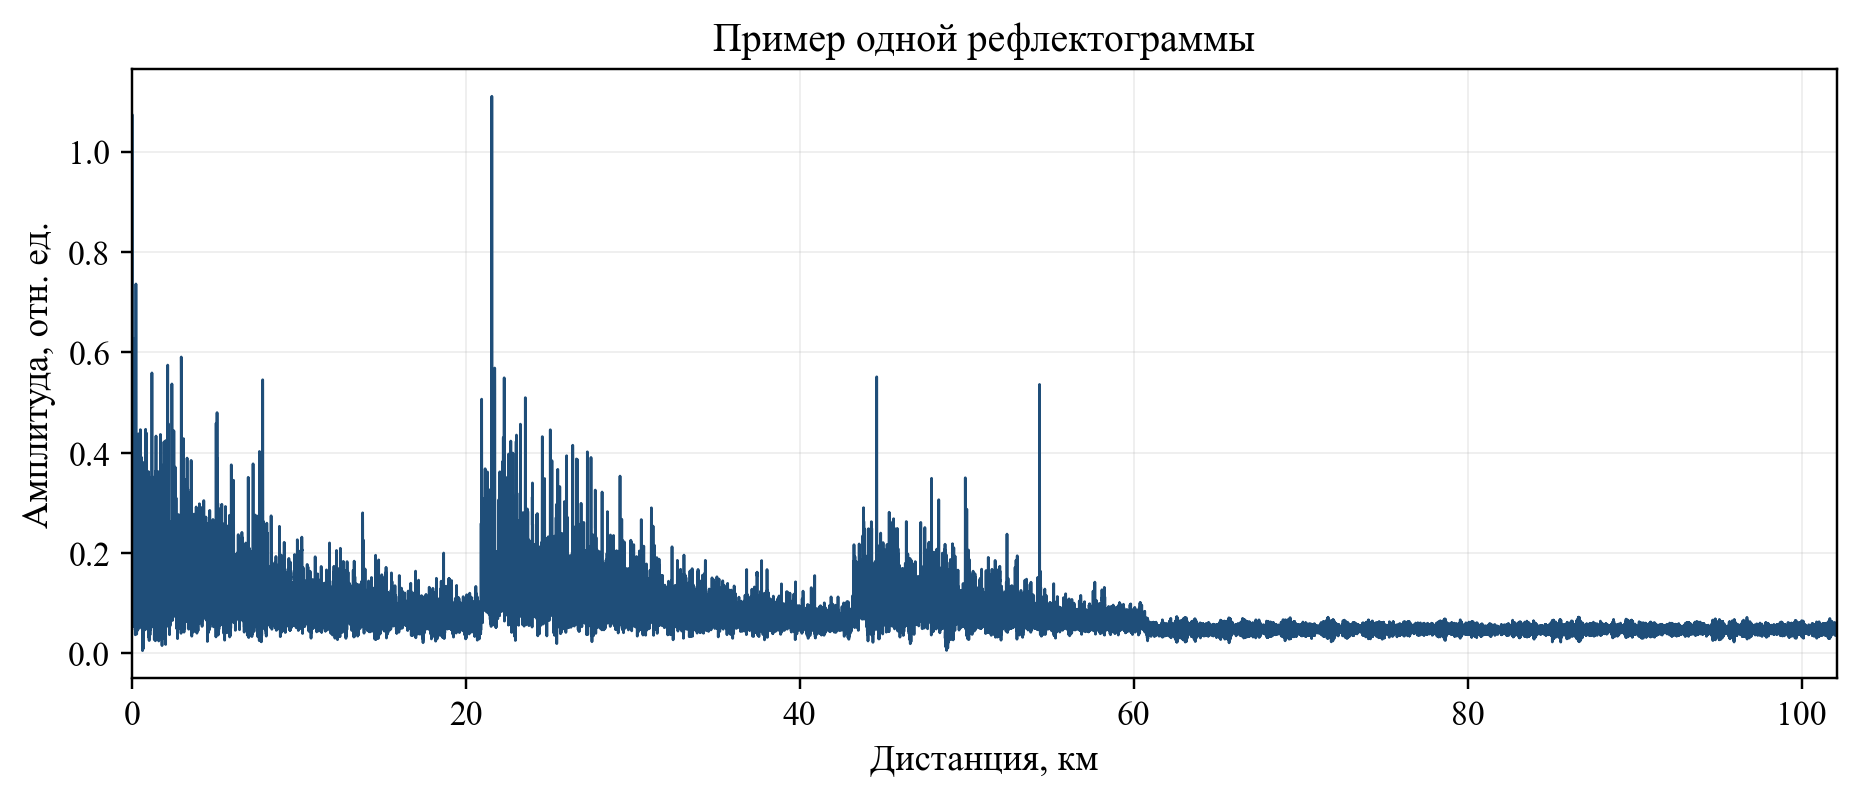
\includegraphics[width=0.92\textwidth]{fig_reflectogram.png}
  \caption{Пример одной рефлектограммы, зарегистрированной на длинной линии с EDFA-усилителями. Видны ступенчатые подъёмы амплитуды на дистанциях 21 км, 43 км и 49 км - точки расположения распределённых усилителей.}
  \label{fig:reflectogram}
\end{figure}

% ---- 2.2 Длинные линии с усилителями ----
\subsection{Особенности длинных линий с распределёнными усилителями}
\label{sec:longline}

При увеличении длины оптической линии до десятков и сотен километров затухание зондирующего сигнала становится принципиальным фактором. Для стандартного одномодового волокна затухание на длине волны 1550~нм составляет около 0{,}2~дБ/км; на линии длиной 60~км обратное рассеяние ослабляется более чем на 24~дБ относительно начального участка. Без активной компенсации регистрируемая амплитуда падает экспоненциально, и шум детектора начинает доминировать на дальних участках линии~\cite{Peng2014, WangZN2014}.

Для увеличения предельной длины линии применяют распределённые оптические усилители: эрбиевые (EDFA) и схемы рамановского усиления~\cite{Martins2014, Wang2016}; экспериментально продемонстрированы phi-OTDR-системы с длинами линий 123~км на двусторонней EDFA-схеме~\cite{Tian2016}, 175~км на гибридной EDFA+Raman-схеме~\cite{WangZN2014}, 190~км и 300~км на оптимизированных каскадах усилителей~\cite{Wang2023, Fan2023}. Такие усилители частично компенсируют затухание сигнала, однако вносят в систему усиленную спонтанную эмиссию (ASE - Amplified Spontaneous Emission), которая на участках, прилегающих к усилителям, заметно повышает фоновый уровень шума. В результате фон обратного рассеяния по дистанции оказывается резко неоднородным: на длинной линии чередуются участки с типичным релеевским шумом и участки с выраженным ASE-шумом усилителей.

Эта неоднородность фона представляет собой принципиальную трудность для классических энергетических детекторов возмущений, оценивающих среднеквадратичную амплитуду по времени для каждой дистанционной точки. Точечные возмущения вблизи усилителя могут оказаться неотличимы от стационарного шума ASE по интегральной энергии. Как будет показано в разделе результатов, простой энергетический детектор на размеченном наборе данных уступает по F1-мере спектральному детектору практически в полтора раза.

% ---- 2.3 Существующие методы локализации ----
\subsection{Существующие методы локализации возмущений}
\label{sec:existing}

В литературе предложено несколько групп методов автоматической локализации возмущений по данным \phiOTDR. Их можно разделить на четыре класса по используемому математическому аппарату и сводный анализ представлен в таблице~\ref{tab:methods}.

\subsubsection*{Непрерывное вейвлет-преобразование (CWT)}

Подход, предложенный Z.~Qin и соавт.~\cite{Qin2012}, основан на построении вейвлет-скалограммы для каждой дистанционной точки и поиске вейвлет-гребня в плоскости (частота, время). Для локализации возмущения используется глобальный спектр энергии гребня по дистанции. Метод хорошо работает на коротких линиях с нестационарными вибрациями (например, импульсные акустические воздействия), однако требует полного двумерного time-frequency анализа для каждой пространственной точки и не учитывает неоднородность фона на длинных линиях с усилителями.

\subsubsection*{Преобразование Гильберта–Хуанга (HHT)}

X.~Hui и соавт.~\cite{Hui2014} использовали преобразование Гильберта–Хуанга для частотно-временного анализа возмущений в \phiOTDR. Эмпирическая модовая декомпозиция (EMD) даёт адаптивное представление сигнала суммой собственных модовых функций, после чего по каждой моде строится мгновенная частота через преобразование Гильберта. Метод позволяет локализовать нестационарные воздействия без априорного задания базиса, как в вейвлет-разложении, однако его выходом также служит двумерное распределение (мода, дистанция); кроме того, эмпирическая декомпозиция чувствительна к артефактам перемежения мод и предъявляет высокие требования к качеству исходного сигнала, что затрудняет её применение на длинной линии с резко неоднородным фоном.

\subsubsection*{Декомпозиция по вейвлет-пакетам}

Q.~Li и соавт.~\cite{Li2014} применили дискретную декомпозицию по вейвлет-пакетам для разделения сигнала по частотным полосам и расчёта энергий пакетов как функции дистанции. Метод устойчив к медленному дрейфу частоты лазера и позволяет одновременно локализовать несколько возмущений, однако выходом метода служит двумерная энергетическая карта (частотный пакет, дистанция), а не компактный одномерный score; интерпретация результата требует дополнительной агрегации, характер которой в работе не зафиксирован.

\subsubsection*{Сопоставление матрицы данных (Data Matrix Matching)}

X.~Liu и соавт.~\cite{Liu2018} предложили метод, в котором для каждой пары соседних трасс вычисляется матрица расстояний и сравнивается с эталоном «спокойного» состояния линии. Метод работает в реальном времени с откликом порядка 50~мс и продемонстрирован на короткой (1{,}2~км) линии. Подход существенно опирается на конкретную схему регистрации и эталонное состояние; неоднородность фона длинной линии при наличии распределённых усилителей в исходной работе не рассматривается.

\subsubsection*{Методы машинного обучения}

В последние годы предложено несколько подходов на основе нейронных сетей. H.~Wu и соавт.~\cite{Wu2019} применили скрытые марковские модели (HMM) для распознавания типа возмущения по последовательности признаков, а Y.~Shi и соавт.~\cite{Shi2020} - свёрточные нейронные сети для классификации событий в \phiOTDR. ML-методы достигают высокой точности классификации при наличии большого размеченного набора данных, но обладают двумя характерными ограничениями. Во-первых, они требуют существенных размеров обучающей выборки (тысячи событий с метками класса), которой в большинстве лабораторных установок \phiOTDR{} нет. Во-вторых, обученная модель не даёт физической интерпретации результата: при ложном срабатывании невозможно понять, какая характеристика сигнала привела к неверному решению.

\begin{table}[h]
\caption{Сравнение четырёх семейств методов локализации возмущений в \phiOTDR.}
\label{tab:methods}
\centering
\renewcommand{\arraystretch}{1.25}
\begin{tabular}{p{3.4cm} p{3.6cm} p{3.4cm} p{3.5cm}}
\toprule
\textbf{Метод} & \textbf{Применимость} & \textbf{Выход} & \textbf{Ограничения} \\
\midrule
CWT~\cite{Qin2012} & Короткие линии, нестационарные импульсы & 2D скалограмма + гребень & Полный 2D-анализ, нет учёта неоднородного фона \\
HHT~\cite{Hui2014} & Нестационарные сигналы, адаптивный базис & 2D распределение (мода, дистанция) & Артефакты перемежения мод, чувствительность к шуму \\
Вейвлет-пакеты~\cite{Li2014} & Стационарные вибрации & 2D карта (пакет, дистанция) & Двумерный выход, требует дополнительной агрегации \\
Сопоставление матриц~\cite{Liu2018} & Короткие линии (1-2 км) & Бинарная карта расстояний & Зависимость от эталона; короткие линии \\
Машинное обучение~\cite{Wu2019, Shi2020} & Классификация событий & Метка класса & Нужна большая разметка, нет интерпретируемости \\
\bottomrule
\end{tabular}
\end{table}

Отдельного внимания заслуживает требование к минимальной длительности окна регистрации. Методы на основе непрерывного вейвлет-преобразования, преобразования Гильберта–Хуанга и декомпозиции по вейвлет-пакетам по построению предполагают наличие достаточно длинного временного окна для полноценного частотно-временного анализа на каждой пространственной точке. В работе~\cite{Qin2012} анализ выполняется на окне порядка нескольких секунд непрерывной регистрации; HHT-разложение в~\cite{Hui2014} и декомпозиция по вейвлет-пакетам в~\cite{Li2014} аналогично требуют тысячи последовательных рефлектограмм для устойчивой оценки амплитуд мод и энергий пакетов. Метод сопоставления матриц~\cite{Liu2018} формально работает на парах соседних трасс, но дальнейшая фильтрация по пространственному смыслу всё же требует усреднения по сотням трасс, к тому же подход опирается на отдельно набранную эталонную запись «спокойного» состояния линии. Методы машинного обучения~\cite{Wu2019, Shi2020} обычно тренируются и применяются на окнах в десятки тысяч трасс.

% ---- 2.4 Постановка задачи ----
\subsection{Постановка задачи}
\label{sec:problem}

Анализ литературы выявляет общий пробел: существующие методы либо ориентированы на короткие линии и не учитывают неоднородность фона при наличии распределённых усилителей, либо выдают результат в виде двумерной карты (частота, дистанция), требующей дополнительной интерпретации. Параллельно методы машинного обучения требуют размеченных данных в объёмах, нехарактерных для лабораторных \phiOTDR-установок, и не дают физически интерпретируемых решений.

Сформулируем требования к разрабатываемому методу:
\begin{enumerate}[leftmargin=2.5em, label=\arabic*.]
  \item \textbf{Устойчивость к затуханию вдоль линии} - необходимо учесть зависимость уровня фона от дистанции, в первую очередь - резкие подъёмы фона вблизи EDFA-усилителей.
  \item \textbf{Независимость от знания частоты воздействия} - метод не должен опираться на априорное знание спектральных характеристик возмущения, поскольку реальные акустические воздействия имеют широкий и заранее неизвестный спектр.
  \item \textbf{Компактный одномерный результат} - выходом детектора должна быть зависимость скалярной оценки $S(g)$ от дистанции, а не 2D-карта в плоскости (частота, дистанция); это упрощает интерпретацию, хранение и пороговый отбор кандидатов.
  \item \textbf{Короткое окно регистрации} - метод должен давать корректную детекцию импульсного воздействия на окне порядка $10^2$ рефлектограмм (около десятых долей секунды на типичном темпе следования зондирующих импульсов), без необходимости в дополнительной эталонной записи «спокойного» состояния линии.
  \item \textbf{Воспроизводимая валидация на размеченном наборе} - метод должен быть оценён по Precision, Recall, F1-мере и медианной ошибке локализации на наборе с известными зонами воздействия, а его выбор аргументирован сопоставлением с одно-компонентными детекторами-эталонами на тех же данных.
\end{enumerate}

\newpage

% =====================================================================
%  3. ДАННЫЕ И МЕТОД
% =====================================================================
\section{Данные и метод}

% ---- 3.1 Описание датасета ----
\subsection{Описание датасета}
\label{sec:dataset}

Все экспериментальные данные получены на лабораторной установке \phiOTDR; настоящая работа использует их как готовый источник и сосредоточена на алгоритмах обработки. Установка работает на длине волны 1550~нм с частотой дискретизации аналого-цифрового преобразователя $F_s = 50$~МГц и пятью значениями длительности зондирующего импульса $\tau \in \{100, 200, 300, 500, 1000\}$~нс. Регистрация ведётся на четырёх физически различных одномодовых оптических линиях с распределёнными EDFA-усилителями; протяжённость линий - от единиц до примерно 60~км.

Полный объём использованных данных - 882 записи общей длительностью около получаса непрерывного наблюдения. По характеру эксперимента записи делятся на четыре категории: записи фонового мониторинга линий (около половины датасета), записи с контролируемым механическим воздействием на участок волокна (около трети), длительные тестовые записи на стационарной линии (около десятой части) и небольшая серия записей со статической растяжкой волокна. Около 60~\% записей содержат непрерывный сигнал с АЦП длительностью около 1~секунды; в остальных случаях запись расширена до 10~секунд для исследования стабильности фона. Около трети датасета представлено в виде уже выделенных последовательностей рефлектограмм, для которых этап парсера не выполняется.

Для количественной валидации метода выделен размеченный поднабор из 130 записей. Разметка получена из протокола эксперимента и для каждой записи указывает либо координаты начала и конца зоны воздействия в метрах вдоль волокна, либо отметку об отсутствии воздействия. На размеченном поднаборе представлены все четыре линии и все пять длительностей импульса. Из 130 записей 92 содержат подтверждённое воздействие (положительные кейсы) и 38 представляют состояние линии без воздействия (отрицательные кейсы).

% ---- 3.2 Парсер ----
\subsection{Парсер: выделение рефлектограмм из сырой записи}
\label{sec:parser}

Из непрерывной записи $x[n]$, $n = 0\dots N-1$, требуется выделить последовательность отдельных рефлектограмм фиксированной длины $\hat{L}$. Основная сложность - установить положение начал импульсов, поскольку период следования и длительность каждой рефлектограммы заранее неизвестны и зависят от настроек установки. Реализованный парсер включает четыре шага.

\textbf{Шаг 1. Прореживание и сглаживание.} Из исходного сигнала $x[n]$, $n = 0, 1, \dots, N-1$, строится сглаженная огибающая $m[n]$ как выпуклая комбинация скользящего среднего и экспоненциальной огибающей по абсолютному значению сигнала $|x[n]|$:
\begin{equation}
  m[n] = \alpha \cdot \mathrm{SMA}_w(|x|)[n] + (1-\alpha) \cdot \mathrm{EMA}_\beta(|x|)[n],
\end{equation}
где $\mathrm{SMA}_w$ - оператор скользящего среднего по окну длины $w$ отсчётов, $\mathrm{SMA}_w(y)[n] = (1/w) \sum_{k=0}^{w-1} y[n-k]$; $\mathrm{EMA}_\beta$ - экспоненциальная скользящая средняя с коэффициентом сглаживания $\beta \in (0, 1)$, заданная рекуррентно как $\mathrm{EMA}_\beta(y)[n] = \beta\,y[n] + (1-\beta)\,\mathrm{EMA}_\beta(y)[n-1]$; $\alpha \in [0, 1]$ - весовой коэффициент. Дополнительно вычисляется первая разность $g[n] = m[n] - m[n-1]$, играющая роль дискретного градиента огибающей.

\textbf{Шаг 2. Устойчивые к выбросам пороги и поиск кандидатов в начала.} Устойчивый к выбросам размах огибающей определяется через эмпирические квантили её распределения:
\begin{equation}
  \Delta = Q_{0{,}98}(m) - Q_{0{,}02}(m),
\end{equation}
где $Q_p(\cdot)$ - эмпирический $p$-й квантиль распределения значений соответствующего сигнала. По размаху $\Delta$ задаются два порога:
\begin{equation}
  \theta_\text{low} = Q_{0{,}02}(m) + \beta_\text{low} \cdot \Delta, \qquad
  \theta_\text{rise} = \beta_\text{rise} \cdot \Delta,
\end{equation}
где $\beta_\text{low}, \beta_\text{rise} \in (0, 1)$ - эмпирически подобранные коэффициенты, фиксирующие положение порогов внутри устойчивого к выбросам размаха. Точка $k$ принимается за кандидата в начало рефлектограммы, если одновременно выполнено $m[k-1] < \theta_\text{low}$ и $g[k] > \theta_\text{rise}$. Применение квантилей вместо среднего и стандартного отклонения делает пороги устойчивыми к выбросам, типичным для участков с воздействием.

\textbf{Шаг 3. Авто-оценка периода.} По множеству кандидатов строится гистограмма попарных интервалов $\{k_{i+1} - k_i\}$. Для каждого пика гистограммы подсчитывается «голос» с весом $1/\sqrt{j}$, где $j$ - гармоника пика по отношению к минимальному периоду. Выбирается период $T^*$, набравший наибольший суммарный вес. Эта схема устойчива к пропущенным начальным точкам: один пропуск даёт «удвоенный» интервал, который автоматически интерпретируется как вторая гармоника.

\textbf{Шаг 4. Восстановление пропусков и финализация.} Между двумя соседними подтверждёнными «якорными» началами $k_a$, $k_b$, расстояние между которыми кратно периоду $T^*$, генерируются недостающие начала с шагом $T^*$. Длина рефлектограммы $\hat{L}$ оценивается как медиана длин подтверждённых пачек. Качество парсинга характеризуется коэффициентом покрытия $K = N_\text{извл}/N_\text{ож}$, где $N_\text{извл}$ - число корректно выделенных рефлектограмм, $N_\text{ож}$ - ожидаемое число рефлектограмм по длительности записи и периоду $T^*$.

% ---- 3.3 Кросс-корреляционное выравнивание ----
\subsection{Кросс-корреляционное выравнивание трасс}
\label{sec:alignment}

Между соседними рефлектограммами наблюдается межтрассовый джиттер на уровне долей и единиц отсчётов АЦП, обусловленный, в частности, тепловым дрейфом задержки в источнике излучения и дискретизацией начала захвата окном. Этот джиттер искажает преобразование Фурье по времени для каждого дистанционного бина и существенно ухудшает качество детектора.

Для каждой $i$-й трассы оценивается целочисленный сдвиг $s_i$ относительно опорной (нулевой) трассы. Сдвиг определяется по положению локального максимума взаимной корреляционной функции в окне дистанционных бинов $[a, a+W]$ ($a$~- начало окна, $W$~- его длина в бинах), выбранном на участке с устойчивым отражением вдоль волокна. Накопленный по всем соседним парам сдвиг агрегируется до абсолютной кривой $\{s_i\}_{i=0}^{N_\text{trace}-1}$, после чего применяется медианная нормировка для подавления глобального дрейфа. Выровненный массив получается покадровым целочисленным сдвигом строк:
\begin{equation}
  \text{aligned}[i, :] = \mathrm{shift}(\text{traces}[i, :], -s_i),
\end{equation}
где $\mathrm{shift}(y, k)$~ - оператор сдвига одномерного массива $y$ на $k$ позиций влево с заполнением освобождающихся отсчётов нулями; $\text{traces}[i, :]$~- $i$-я строка исходного массива рефлектограмм.

Для предотвращения деградации качества при ошибочной оценке сдвигов введены три критерия приёма выравнивания. Пусть $r_i$~- невязка $i$-й трассы относительно опорной (среднеквадратичное отклонение по дистанционным бинам в общем окне), $\langle r \rangle$~- среднее значение $r_i$ по всем трассам записи, $r_{p95}$~- 95-й перцентиль распределения $r_i$ по трассам, $\rho_{q99}$~- 99-й перцентиль распределения попарных разностей соседних трасс по дистанции (мера межтрассовой шероховатости). Выравнивание принимается, если выполнено хотя бы одно из условий:
\begin{enumerate}[leftmargin=2.5em, label=(\arabic*)]
  \item $\langle r \rangle_\text{after} \le 0{,}92 \cdot \langle r \rangle_\text{before}$~ - снижение средней невязки не менее чем на 8\%;
  \item $r_{p95}^\text{after} \le 0{,}70 \cdot r_{p95}^\text{before}$ при росте стандартного отклонения не более чем на 5\%~- улучшение хвоста распределения невязки;
  \item $\rho_{q99}^\text{after} \le 0{,}90 \cdot \rho_{q99}^\text{before}$~ - снижение межтрассовой шероховатости не менее чем на 10\%.
\end{enumerate}
Индексы $\text{before}$ и $\text{after}$ обозначают значение соответствующей величины до и после применения сдвигов. Если ни одно из трёх условий не выполнено, выравнивание отклоняется и используется исходный массив. На рис.~\ref{fig:waterfall} показана водопадная диаграмма после успешного выравнивания на одной из положительных размеченных записей (длительность около 1~секунды).

\begin{figure}[h]
  \centering
  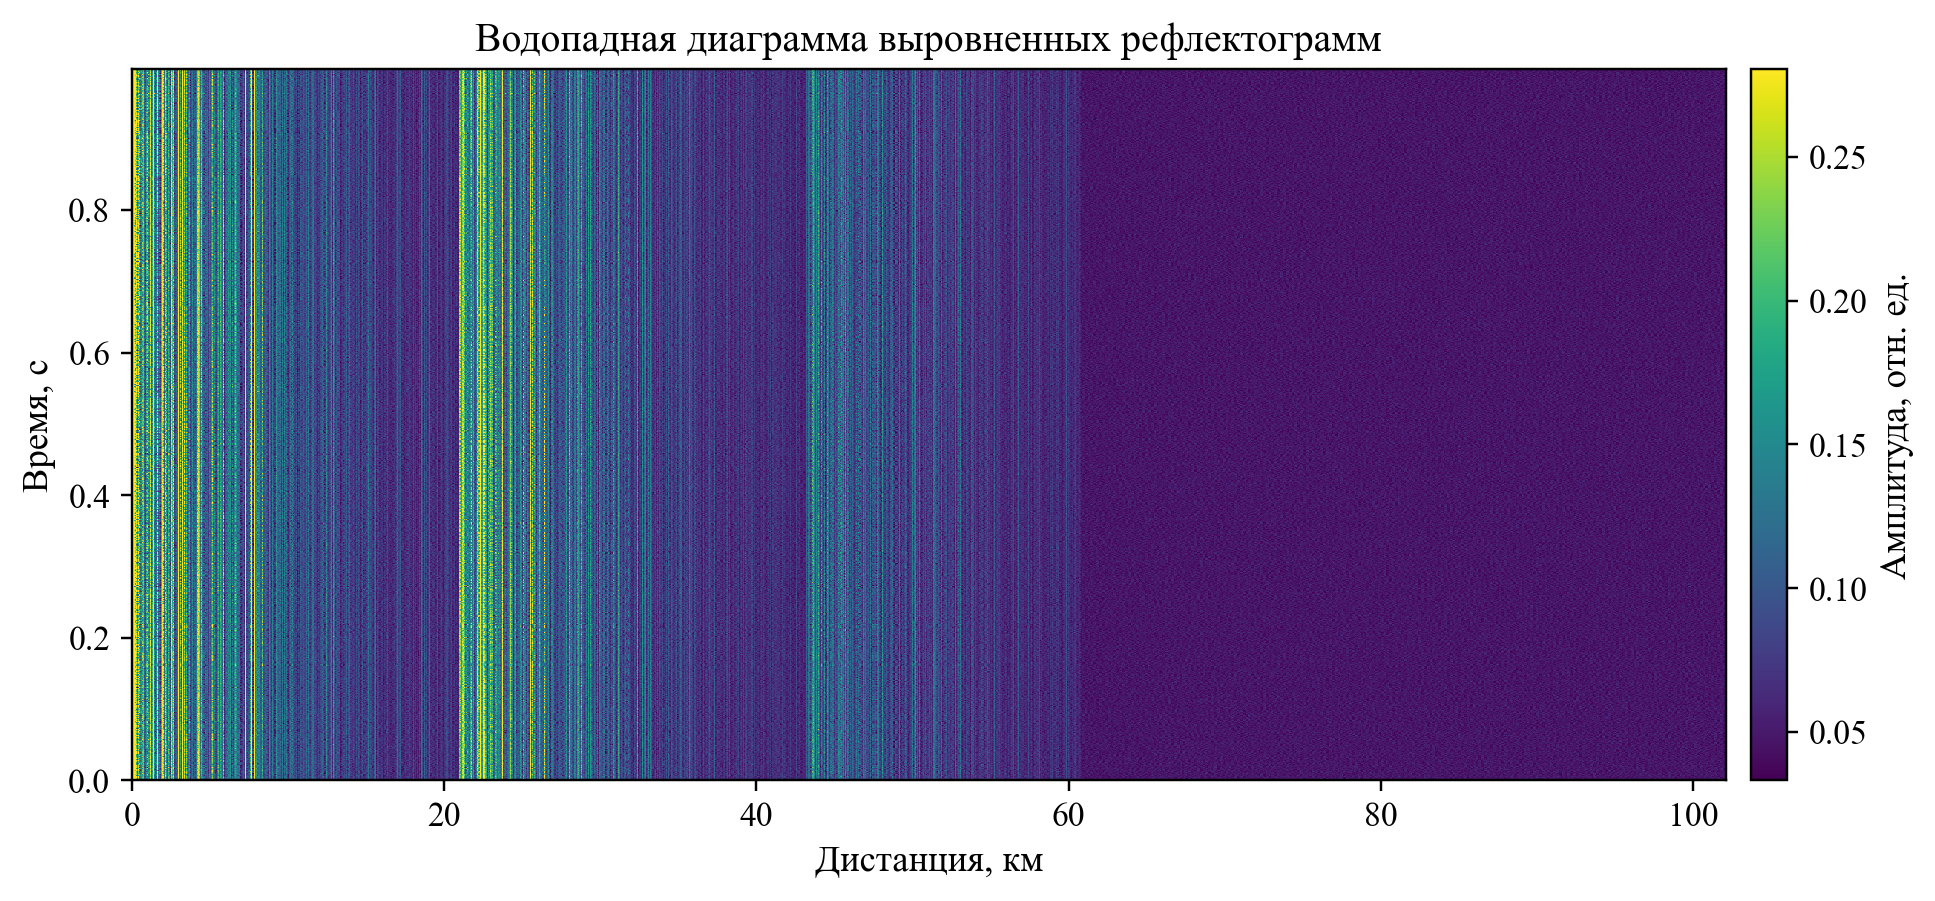
\includegraphics[width=0.92\textwidth]{fig_waterfall_aligned.png}
  \caption{Водопадная диаграмма выровненных рефлектограмм. По вертикальной оси отложено время регистрации (около 1~с непрерывной записи), по горизонтальной - дистанция вдоль волокна. Видна полезная зона до 60~км и шумовая зона после.}
  \label{fig:waterfall}
\end{figure}

% ---- 3.4 Устойчивый к выбросам детектор ----
\subsection{Устойчивый к выбросам детектор возмущений}
\label{sec:detector}

Детектор представляет собой последовательность из шести шагов, преобразующих выровненный массив $\text{aligned}[t, d]$ размерности $[N_\text{trace} \times N_\text{dist}]$ в одномерную оценку $S(g)$ по сгруппированным дистанционным бинам, по которой затем производится пороговый отбор кандидатов. Здесь и далее $t \in \{0, \dots, N_\text{trace}-1\}$~- индекс трассы (по времени), $d \in \{0, \dots, N_\text{dist}-1\}$~- индекс дистанционного бина, $g$~- индекс группы дистанционных бинов; нижний индекс у статистических операторов (например, $\mathrm{med}_t$, $\mathrm{MAD}_g$) обозначает ось, по которой выполняется операция.

\textbf{Шаг 1. Медианный фон и вычитание.} Стационарный фон линии оценивается медианой по времени независимо для каждого дистанционного бина:
\begin{equation}
  B(d) = \mathrm{med}_t \, \text{aligned}[t, d], \qquad
  R[t, d] = \text{aligned}[t, d] - B(d),
\end{equation}
где $B(d)$~ - оценка фона в дистанционной точке $d$, $\mathrm{med}_t$~ - медиана по индексу $t$ (по времени), $R[t, d]$~ - остаток рефлектограммы относительно фона. Использование медианы вместо среднего обеспечивает устойчивость оценки фона к импульсным выбросам в местах активного воздействия.

\textbf{Шаг 2. MAD-нормировка по дистанции.} Для каждого дистанционного бина оценивается устойчивый к выбросам масштаб $\sigma(d)$ через медианное абсолютное отклонение (MAD~ - Median Absolute Deviation):
\begin{equation}
  \sigma(d) = 1{,}4826 \cdot \mathrm{med}_t \,\big| R[t, d] - \mathrm{med}_t R[t, d] \big|,
\end{equation}
где коэффициент $1{,}4826 \approx 1/\Phi^{-1}(0{,}75)$ ($\Phi$~ - функция распределения стандартной нормальной случайной величины) обеспечивает асимптотическую несмещённость оценки $\sigma(d)$ относительно стандартного отклонения нормально распределённой величины~\cite{Hampel1974}. Нормированный по дистанции остаток
\begin{equation}
  z[t, d] = R[t, d] / \sigma(d)
\end{equation}
имеет масштаб порядка единицы на участках без активности и достигает значений 5-10 в местах воздействий.

\textbf{Шаг 3. Группировка по дистанции и преобразование Фурье по времени.} Для снижения шума и вычислительной нагрузки соседние дистанционные бины объединяются в неперекрывающиеся группы по $G = 20$ бинов (что соответствует пространственной апертуре около 40~м):
\begin{equation}
  \tilde{z}(t, g) = \frac{1}{G}\sum_{d \in \mathcal{G}_g} z[t, d],
\end{equation}
где $\mathcal{G}_g$~ - множество индексов дистанционных бинов, попавших в группу $g$, $\tilde{z}(t, g)$~ - сгруппированный нормированный сигнал. К нему применяется быстрое преобразование Фурье $\mathrm{FFT}_t$ по оси времени отдельно для каждой группы $g$, после чего квадрат модуля нормируется на длину последовательности и переводится в логарифмический масштаб:
\begin{equation}
  P(f, g) = 10\,\lg \frac{\big|\,\mathrm{FFT}_t \tilde{z}(t, g)\,\big|^2}{N_\text{trace}},
\end{equation}
где $f$~- частота (выходная переменная преобразования Фурье), $N_\text{trace}$~- число трасс в записи, $P(f, g)$~ - спектральная плотность мощности в децибелах.

\textbf{Шаг 4. Устойчивая к выбросам нормировка по частоте.} В каждой частотной строке $f$ оценивается медиана и MAD значений $P(f, g)$ по оси групп и формируется z-оценка спектра:
\begin{equation}
  z_f(f, g) = \frac{P(f, g) - \mathrm{med}_g P(f, g)}{1{,}4826 \cdot \mathrm{med}_g \big|P(f, g) - \mathrm{med}_g P(f, g)\big|},
\end{equation}
где $\mathrm{med}_g$~- медиана по индексу группы $g$, $z_f(f, g)$~- нормированный спектр. Эта операция компенсирует систематическую неоднородность спектральной плотности по дистанции (в первую очередь повышенный фон ASE вблизи усилителей) и приводит спектр к единому масштабу z-оценок. Используется частотный диапазон $f \in [5,\,F_\text{Nyquist}]$~Гц; нижняя граница исключает медленный дрейф уровня, верхняя~- частота Найквиста для темпа следования рефлектограмм.

\textbf{Шаг 5. Скаляризация: одномерная оценка по дистанции.} Из двумерного массива $z_f(f, g)$ извлекаются три компоненты~- по одной на каждую группу $g$:
\begin{align}
  \mathrm{peak}(g) &= \max_f z_f(f, g), \\
  \mathrm{broad}(g) &= \langle \max(0,\, z_f(f, g) - 1) \rangle_f, \\
  \mathrm{energy\_z}(g) &= \frac{\mathrm{RMS}_t \tilde{z}(t, g) - \mathrm{med}_g \mathrm{RMS}_t \tilde{z}(t, g)}{1{,}4826 \cdot \mathrm{MAD}_g \, \mathrm{RMS}_t \tilde{z}(t, g)},
\end{align}
где $\langle \cdot \rangle_f$~- среднее по частотной оси; $\mathrm{RMS}_t y(t, g) = \sqrt{(1/N_\text{trace}) \sum_t y(t, g)^2}$~- среднеквадратичное значение по времени; $\mathrm{MAD}_g$~- медианное абсолютное отклонение по оси групп. Компонента $\mathrm{peak}(g)$ отвечает за наличие узкого спектрального максимума, $\mathrm{broad}(g)$~- за широкополосную активность (среднюю избыточность z-оценки спектра над уровнем единицы), $\mathrm{energy\_z}(g)$~- за интегральную энергию во временной области, нормированную по дистанции устойчивым к выбросам способом. Комбинированная оценка $S(g)$ формируется как линейная комбинация:
\begin{equation}
  S(g) = 0{,}55 \cdot \mathrm{peak}(g) + 0{,}30 \cdot \mathrm{broad}(g) + 0{,}15 \cdot \mathrm{energy\_z}(g).
  \label{eq:combined}
\end{equation}
Веса $0{,}55$, $0{,}30$ и $0{,}15$ подобраны эмпирически на пилотных записях; в разделе~\ref{sec:ablation} показано, что замена комбинированной оценки $S(g)$ на любую из трёх компонент по отдельности существенно ухудшает F1-меру.

Кривые трёх компонент и комбинированной оценки приведены на рис.~\ref{fig:score_components}. Иллюстрация дана для одной из положительных размеченных записей с двумя зонами контролируемого механического воздействия на расстояниях около 32~км и 42~км от начала линии; эти зоны выделены жёлтыми полосами на всех четырёх панелях.

\begin{figure}[h]
  \centering
  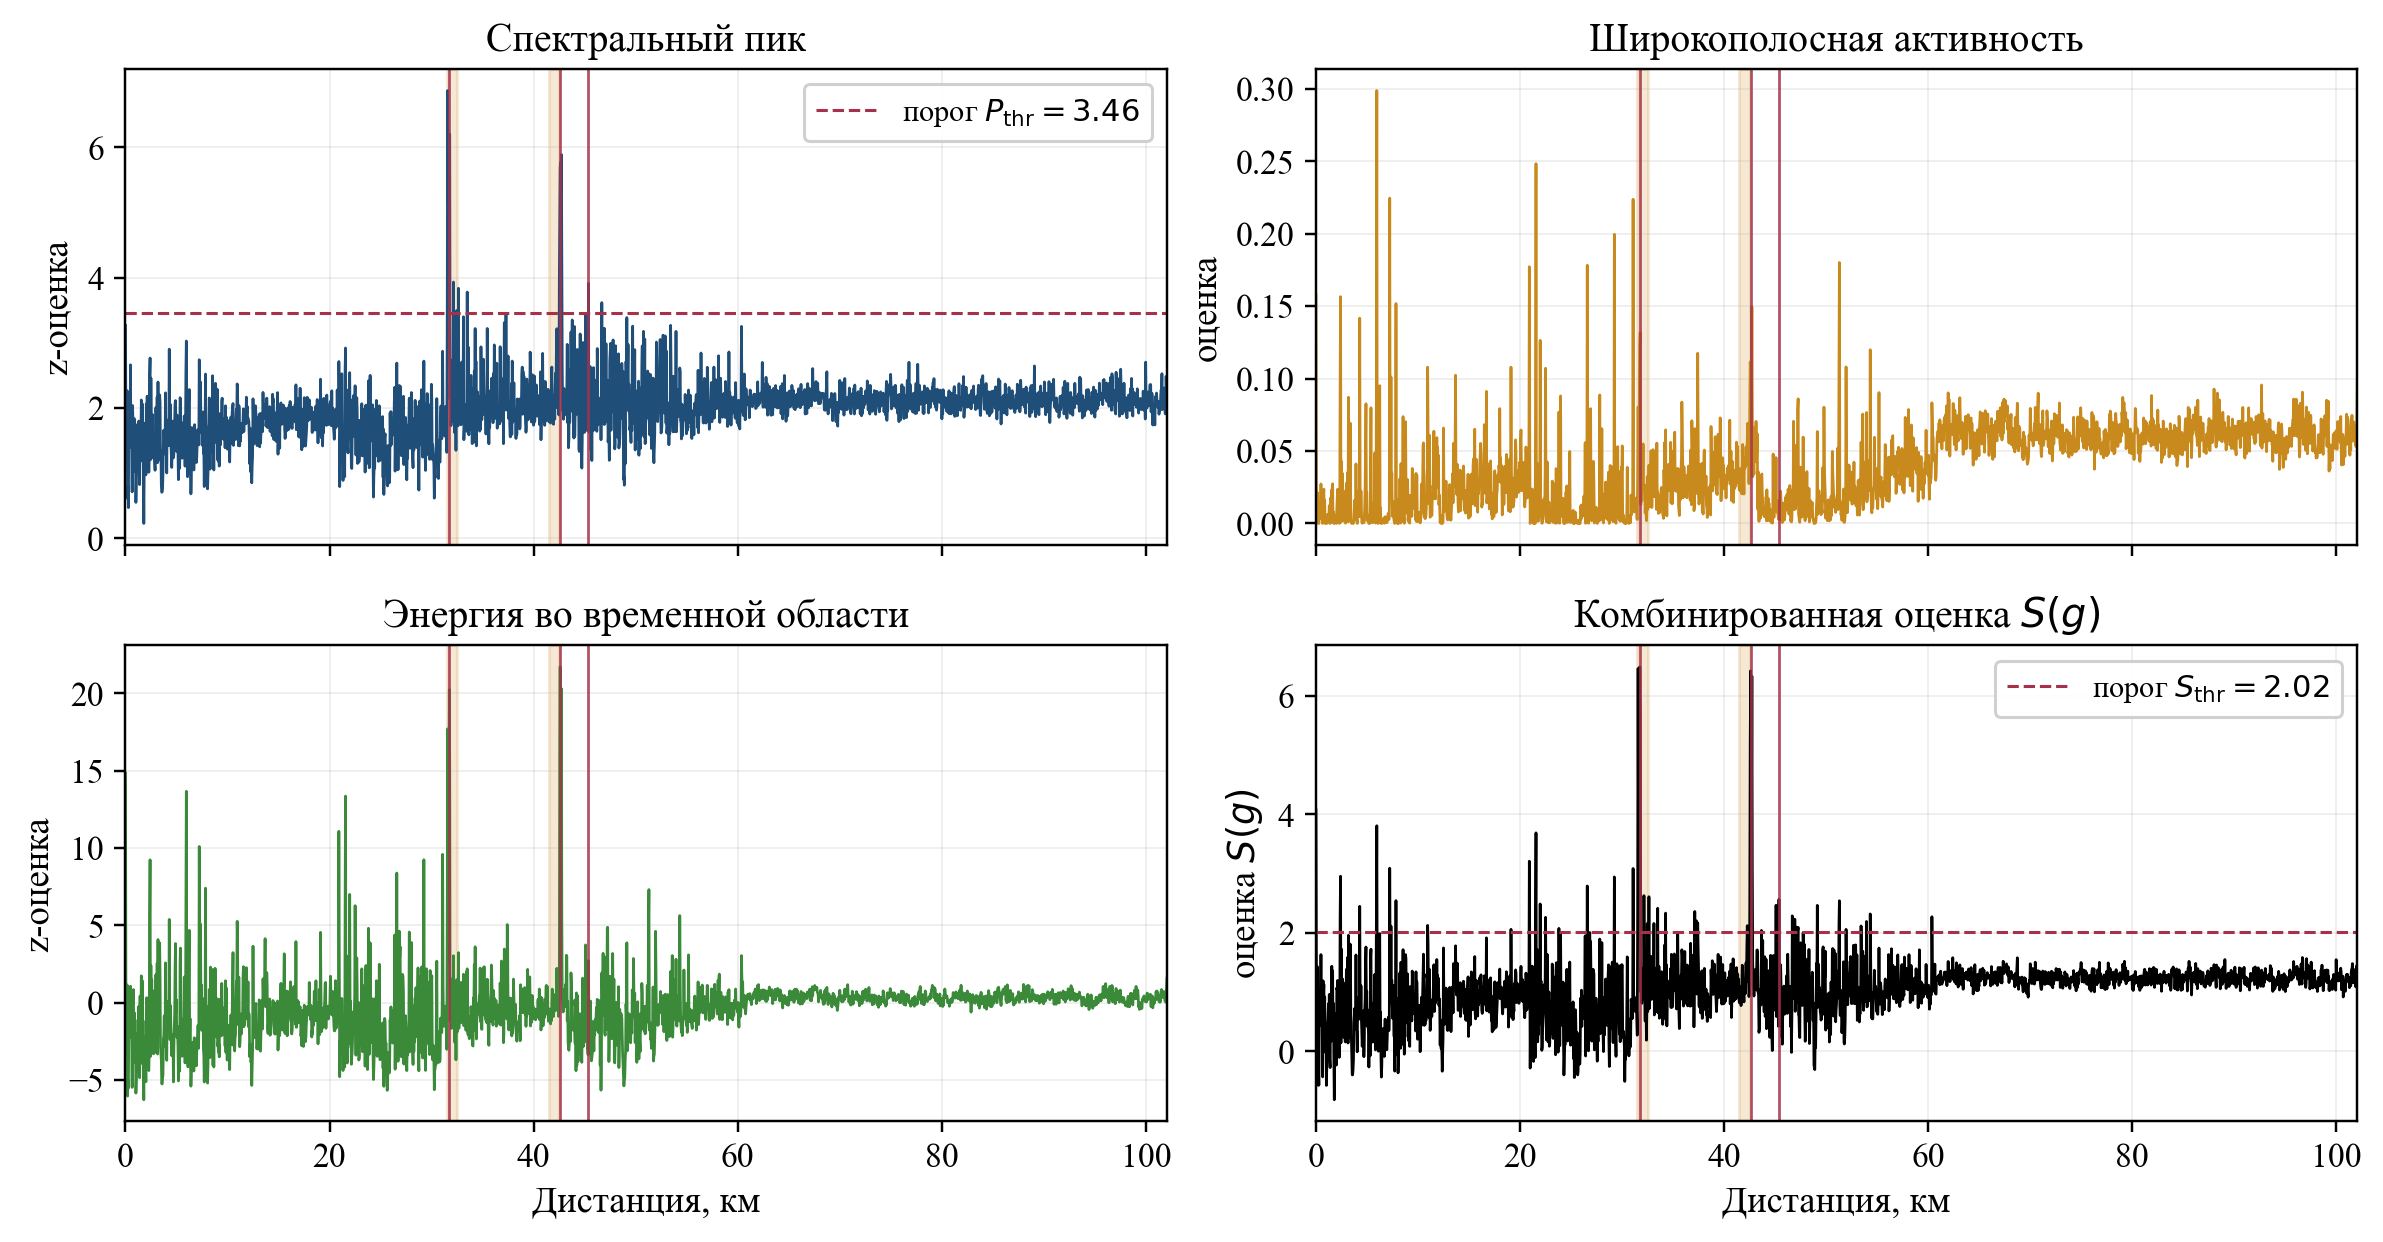
\includegraphics[width=0.98\textwidth]{fig_score_components.png}
  \caption{Спектральные компоненты $\mathrm{peak}(g)$, $\mathrm{broad}(g)$, $\mathrm{energy\_z}(g)$ и их линейная комбинация $S(g)$ на эталонной размеченной записи с двумя зонами контролируемого механического воздействия (около 32~км и 42~км). Красные пунктирные линии на верхней левой и нижней правой панелях - пороги $P_\text{thr}$ и $S_\text{thr}$ соответственно; жёлтые полосы - эталонные зоны воздействия с допуском $\pm 0{,}5$~км; красные сплошные вертикальные линии - три детекции, прошедшие двойной пороговый отбор, на координатах 31{,}7, 42{,}6 и 45{,}4~км (первые две - попадания в эталонные зоны, третья - срабатывание вне зон разметки).}
  \label{fig:score_components}
\end{figure}

\textbf{Шаг 6. Двойной пороговый отбор и подавление повторов.} По распределению $S(g)$ и $\mathrm{peak}(g)$ по всем дистанционным группам оцениваются медиана и MAD, по которым задаются два независимых порога:
\begin{align}
  S_\text{thr} &= \mathrm{med}_g S + 3 \cdot \mathrm{MAD}_g S, \\
  P_\text{thr} &= \mathrm{med}_g \mathrm{peak} + 5 \cdot \mathrm{MAD}_g \mathrm{peak},
\end{align}
где $S_\text{thr}$~- порог по комбинированной оценке, $P_\text{thr}$~- порог по спектральному пику. Группа $g$ отмечается как кандидат, если выполнено сразу два условия
\[
  S(g) \ge S_\text{thr} \quad \text{и} \quad \mathrm{peak}(g) \ge P_\text{thr},
\]
а также $g$ лежит в полезной зоне $[d_\text{ignore},\, d_\text{usable}]$, где $d_\text{ignore}$~- начало полезной зоны (исключаются первые сотни метров с засветкой от выходного импульса лазера), $d_\text{usable}$~- её конец (зона, на которой амплитуда фона ещё не упала до уровня шума детектора). Двойной порог принципиально важен: одиночный порог по $S(g)$ часто срабатывает на участках с повышенным широкополосным шумом, не имеющих узкого спектрального пика; одиночный порог по $\mathrm{peak}(g)$, наоборот, часто срабатывает на стационарных артефактах усилителей.

После порогового отбора применяется подавление повторов: из множества кандидатов выбирается группа с максимальным $S(g)$, после чего удаляются все кандидаты, удалённые от выбранной на расстояние менее $\Delta_\text{min} = 2$~км; процедура повторяется, пока множество не исчерпается. Параметр $\Delta_\text{min}$ задаёт минимальное допустимое расстояние между двумя соседними детекциями.

\textit{Чувствительность к широкополосным возмущениям.} Введение жёсткого порога $P_\text{thr} = 5\,\mathrm{MAD}$ на $\mathrm{peak}(g)$ потенциально ограничивает чувствительность к возмущениям, не порождающим узких спектральных особенностей, - например, локальному нагреву волокна или плавной деформации. На практике эта опасность реализуется лишь для возмущений с полностью диффузным спектром, равномерно распределённым по всему наблюдаемому диапазону. Реальные физические события, представляющие практический интерес для системы (механические импульсы, проезд транспорта, удары и шаги по грунту), даже при формально широкополосной природе порождают неравномерный спектр с одной или несколькими выделенными частотными зонами, обусловленными резонансами в системе грунт - кабель - волокно либо характерными частотами источника воздействия. Соответствующий $\mathrm{peak}(g)$ для таких событий устойчиво превышает $P_\text{thr}$ за счёт $\max$-агрегации по частотным бинам. Чисто диффузные возмущения, не дающие никакой спектральной структуры (например, медленный равномерный нагрев участка волокна), действительно остаются за пределами проектной области предложенного детектора; для их регистрации требуется отдельная стратегия, основанная на сравнении долговременных средних амплитуд $B(d)$ с эталонной записью либо анализе нижней частотной полосы $f < 5$~Гц, исключаемой текущей маской.

С другой стороны, эта же нечувствительность к медленным диффузным изменениям является и преимуществом метода в реальной эксплуатации. Изменение внешних условий, влияющее на всю линию как целое, - например, суточный ход температуры окружающей среды, плавный дрейф мощности лазера или фоновое усиление в EDFA - не порождает узких спектральных особенностей в полосе $f \ge 5$~Гц и не вызывает срабатывания детектора. Иными словами, тёплый день, в течение которого температура грунта над кабелем меняется на 10~K, не приводит к непрерывным ложным детекциям; та же зависимость от $\mathrm{peak}$-признака, которая ограничивает покрытие класса диффузных возмущений, потенциально снижает уровень ложных срабатываний, обусловленных естественными фоновыми процессами. Подчеркнём, что речь идёт именно о качественном механизме фильтрации, а не о количественной оценке Precision в режиме длительного мониторинга: точное значение Precision в реальной эксплуатации зависит от состава отрицательных кейсов и должно отдельно валидироваться на расширенном наборе записей с разных линий и при разных длительностях зондирующего импульса (см. также раздел~\ref{sec:limitations}).

\newpage

% =====================================================================
%  4. РЕЗУЛЬТАТЫ И ОБСУЖДЕНИЕ
% =====================================================================
\section{Результаты и обсуждение}

% ---- 4.1 Качество парсинга ----
\subsection{Качество парсинга}
\label{sec:parser_quality}

Парсер запущен на полном наборе из 552 непрерывных записей аналого-цифрового преобразователя; 330 ранее выделенных последовательностей рефлектограмм добавлены к индексу без выполнения этапа парсера. Из 552 непрерывных записей корректно извлечены 535 (96{,}9\,\%); 17 записей отброшены, поскольку их длительность недостаточна для устойчивой оценки периода следования зондирующих импульсов по гистограмме интервалов (требуется не менее 3-4 пачек рефлектограмм). Сводная статистика по категориям эксперимента приведена в таблице~\ref{tab:parser_summary}.

\begin{table}[h]
\caption{Сводная статистика качества парсинга по категориям эксперимента.}
\label{tab:parser_summary}
\centering
\renewcommand{\arraystretch}{1.15}
\begin{tabular}{p{5.6cm} r r r r r r}
\toprule
\textbf{Категория записей} & \textbf{всего} & \textbf{ok} & \textbf{ok, \%} & \textbf{align, \%} & \textbf{$r_\text{after}$, мед.} & \textbf{$r_\text{after}^{p90}$} \\
\midrule
Записи фонового мониторинга линий & 286 & 286 & 100{,}0 & 73{,}4 & 0{,}00 & 1{,}80 \\
Записи с контролируемым воздействием & 161 & 157 & 97{,}5 & 84{,}7 & 0{,}01 & 12{,}18 \\
Длительные тестовые записи (около 10~с) & 95 & 89 & 93{,}7 & 51{,}7 & 20{,}04 & 51{,}47 \\
Записи со статической растяжкой волокна & 10 & 3 & 30{,}0 & 66{,}7 & 0{,}00 & 0{,}00 \\
\midrule
\textbf{Сырые записи суммарно} & \textbf{552} & \textbf{535} & \textbf{96{,}9} & \textbf{73{,}3} & - & - \\
\bottomrule
\end{tabular}
\end{table}

\noindent
Столбцы таблицы~\ref{tab:parser_summary}:
\begin{itemize}[leftmargin=2em, itemsep=2pt, topsep=2pt]
  \item \textbf{всего} - число записей в категории;
  \item \textbf{ok} - число записей, для которых парсер успешно выделил последовательность рефлектограмм без ошибок;
  \item \textbf{ok, \%} - отношение \textbf{ok}/\textbf{всего} в процентах;
  \item \textbf{align, \%} - доля записей в категории, для которых выравнивание было принято (выполнен хотя бы один из трёх критериев приёма, см. раздел~\ref{sec:alignment}); на остальных записях используется исходный массив без сдвига;
  \item $\mathbf{r_\text{after}}$, \textbf{медиана} - медиана по записям категории среднеквадратичной невязки трасс относительно опорной после выравнивания, в отсчётах АЦП;
  \item $\mathbf{r_\text{after}^{p90}}$ - 90-й перцентиль той же невязки по записям категории; характеризует худшие $10$~\% записей и чувствителен к редким случаям, когда выравнивание не сходится.
\end{itemize}

Категория длительных тестовых записей выделяется существенно более высокой невязкой после выравнивания - медиана $r_\text{after} = 20$ отсчётов вместо нулевой в остальных категориях, и 51 запись из 89 имеют $r_\text{after} > 5$. Это записи длительностью около 10~секунд, в которых фон линии заметно дрейфует во времени; стационарная медианно-MAD модель из раздела~\ref{sec:detector} перестаёт быть адекватной, и качество детектора на таких записях ниже. Подробнее это ограничение рассмотрено в разделе~\ref{sec:limitations}.

% ---- 4.2 Контрольный кейс ----
\subsection{Контрольный кейс на эталонной размеченной записи}
\label{sec:reference}

Для иллюстрации работы детектора рассмотрим одну из положительных размеченных записей длительностью около 1~секунды, на которой по протоколу эксперимента известны два контролируемых воздействия - на расстояниях около 32~км и 42~км от начала линии. На рис.~\ref{fig:final_detection} приведена комбинированная оценка $S(g)$ по дистанции, рассчитанные пороги, эталонные зоны (выделены жёлтым) и детекции, прошедшие двойной пороговый отбор.

\begin{figure}[h]
  \centering
  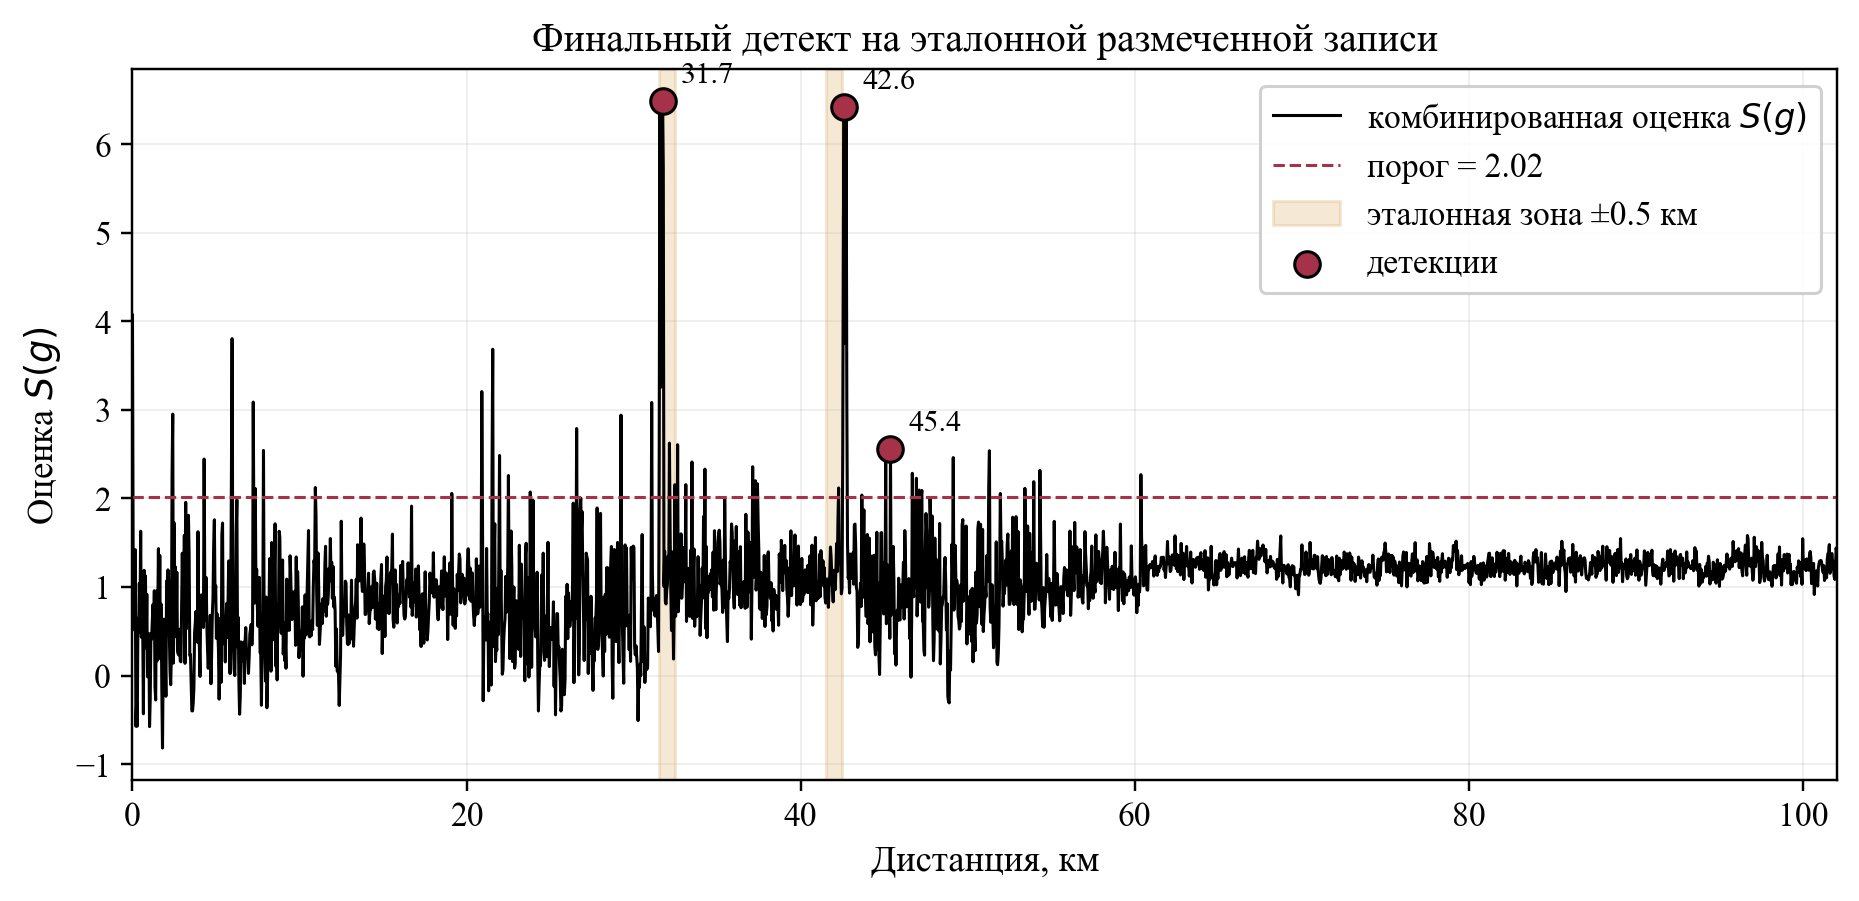
\includegraphics[width=0.95\textwidth]{fig_final_detection.png}
  \caption{Финальный детект на эталонной размеченной записи с двумя контролируемыми воздействиями. Чёрная линия - комбинированная оценка $S(g)$, красный пунктир - порог $S_\text{thr}$, жёлтые полосы - эталонные зоны воздействия с допуском $\pm 0{,}5$~км, кружки - детекции, прошедшие двойной пороговый отбор.}
  \label{fig:final_detection}
\end{figure}

\noindent
Согласно процедуре оценки, детекция засчитывается как попадание в эталонную зону, если её координата $d$ лежит в интервале $[\text{event\_start} - 0{,}5,\, \text{event\_end} + 0{,}5]$~км относительно границ размеченной зоны (правило допуска $\pm 0{,}5$~км вокруг границ); любая детекция вне этих интервалов на положительном кейсе и любая детекция на отрицательном кейсе учитываются как ложное срабатывание (FP) в счётчике Precision. Ошибка локализации для попаданий измеряется как расстояние от детекции до середины зоны $(event\_start + event\_end)/2$ и используется только для отчёта, на бинарное решение «попадание/FP» не влияет. Применяя это правило к рассматриваемой записи, детектор формирует три кандидата: 31{,}7~км (попадание в первую эталонную зону), 42{,}6~км (попадание во вторую эталонную зону) и 45~км (срабатывание вне любой из эталонных зон, засчитанное как FP в общем счётчике из 20 ложных срабатываний по всему размеченному набору). Третья детекция отражает естественную чувствительность детектора к локальным особенностям линии, но без отдельной разметки она не отделима от «настоящего» возмущения и учитывается стандартным способом.

Отдельно стоит отметить, что детектор корректно работает уже на очень малом числе рефлектограмм. Рис.~\ref{fig:short_window} показывает результат при ограничении входа первыми 100 рефлектограммами той же эталонной записи, что соответствует примерно 0{,}1~секунды непрерывного наблюдения линии. Обе размеченные зоны воздействия (около 32~км и 42~км) уверенно выделяются с тем же относительным запасом над порогом, что и на полной односекундной записи; пороги $S_\text{thr}$ и $P_\text{thr}$ слегка снижаются из-за меньшего объёма выборки для оценки устойчивых к выбросам статистик, но контраст между сигналом и фоном остаётся практически тем же. Это означает, что для детекции одиночного импульсного воздействия методу достаточно $\sim 10^2$ периодов следования зондирующих импульсов, что существенно меньше окон, используемых в методах на основе непрерывного вейвлет-преобразования и сопоставления матриц данных (см. раздел~\ref{sec:existing}).

\begin{figure}[h]
  \centering
  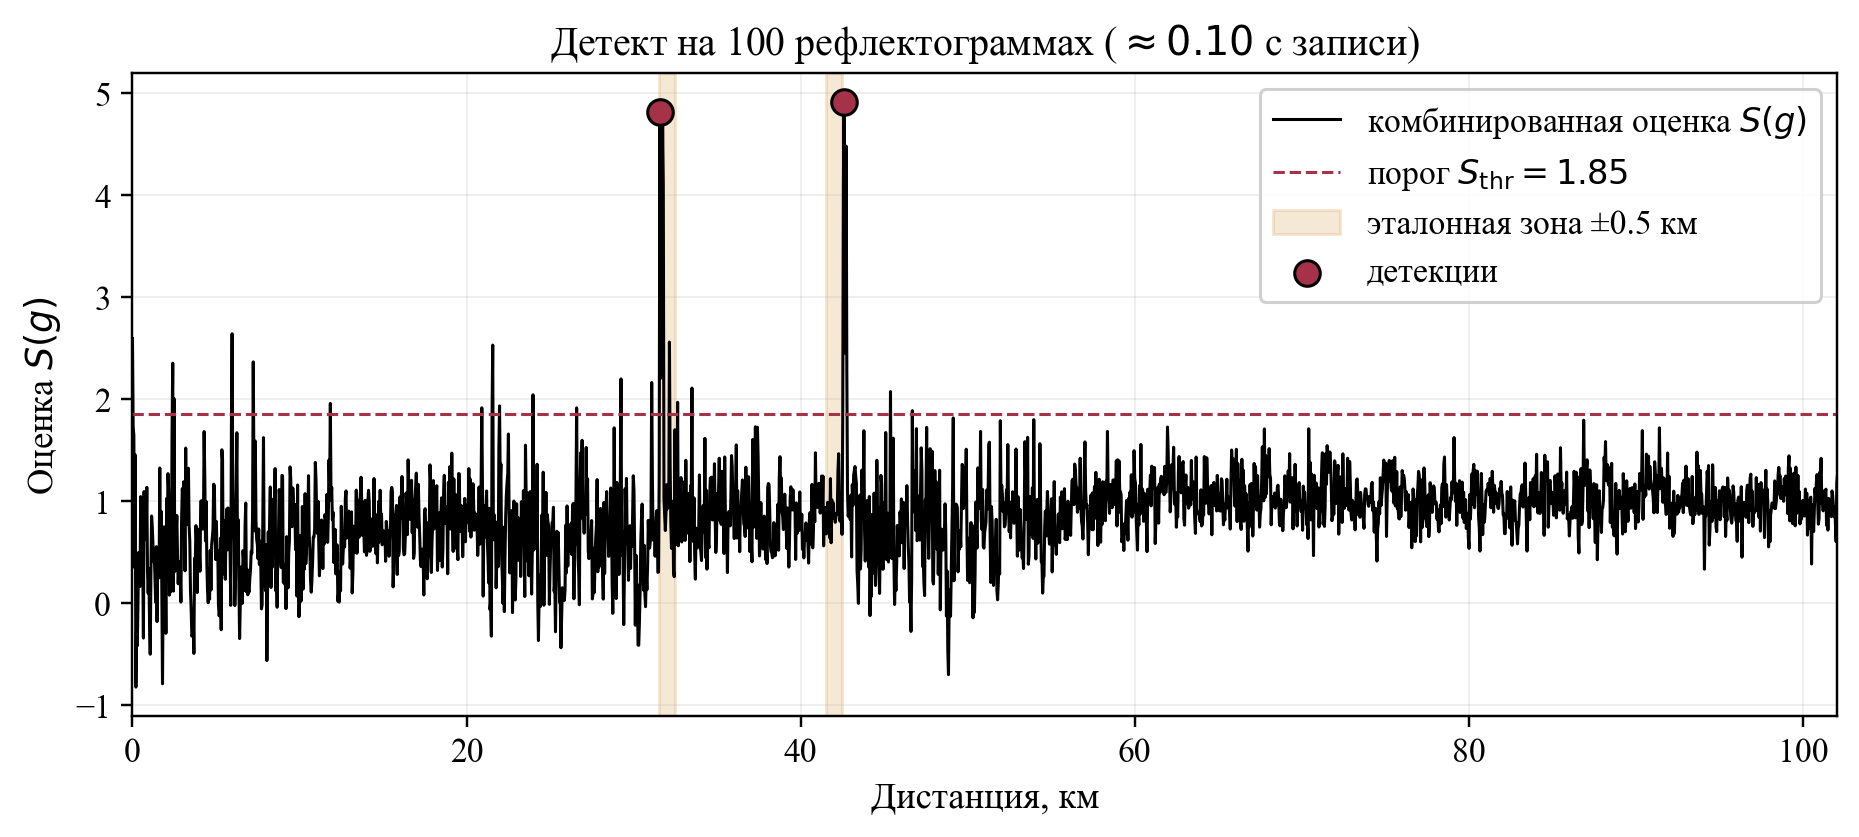
\includegraphics[width=0.92\textwidth]{fig_short_window_100.png}
  \caption{Комбинированная оценка $S(g)$ на той же эталонной записи, но при ограничении входа первыми 100 рефлектограммами (около 0{,}1~секунды записи). Обе эталонные зоны воздействия (около 32~км и 42~км) уверенно выделяются: пиковые значения $S(g)$ более чем в 2{,}5 раза превышают порог $S_\text{thr}$, ни одного ложного срабатывания за пределами эталонных зон не наблюдается.}
  \label{fig:short_window}
\end{figure}

% ---- 4.3 Метрики на 130 файлах ----
\subsection{Метрики на размеченном наборе}
\label{sec:metrics}

Детектор запущен на всех 130 размеченных файлах при едином наборе гиперпараметров: $G = 20$, $f_\text{min} = 5$~Гц, $\Delta_\text{min} = 2$~км, $S_\text{thr} = \mathrm{med} + 3\,\mathrm{MAD}$, $P_\text{thr} = \mathrm{med} + 5\,\mathrm{MAD}$. Правило бинарного решения: детекция засчитывается как попадание, если её координата $d \in [\text{event\_start} - 0{,}5,\, \text{event\_end} + 0{,}5]$~км (допуск $\pm 0{,}5$~км вокруг границ размеченной зоны); все остальные детекции - ложные срабатывания (FP). Ошибка локализации (для попаданий) вычисляется отдельно как расстояние от детекции до середины зоны $(event\_start + event\_end)/2$ и используется только для отчёта. Результаты сведены в таблицу~\ref{tab:main_metrics}.

\begin{table}[h]
\caption{Метрики комбинированного детектора на размеченном наборе.}
\label{tab:main_metrics}
\centering
\renewcommand{\arraystretch}{1.2}
\begin{tabular}{l r}
\toprule
\textbf{Метрика} & \textbf{Значение} \\
\midrule
Recall (порог) & 0{,}380 (35/92) \\
Precision (порог) & 0{,}636 (FP $= 20$) \\
F1-мера (порог) & \textbf{0{,}476} \\
Recall (топ-кандидат) & 0{,}467 (43/92) \\
Медианная ошибка локализации (попадания) & 61~м \\
\bottomrule
\end{tabular}
\end{table}

\noindent
Различим два режима оценки. В первом (\textit{пороговый}) учитываются только те детекции, что прошли двойной пороговый отбор; во втором (\textit{топ-кандидат}) для каждого файла рассматривается группа с максимальной комбинированной оценкой $S(g)$ в полезной зоне, без проверки порога. Recall в режиме порога ниже (0{,}380), но Precision существенно выше; в режиме топ-кандидата Recall достигает 0{,}467, что характеризует предельные возможности метода без зависимости от выбранного порога.

Распределение ошибки локализации показано на рис.~\ref{fig:loc_err_hist}: в режиме порога 31 из 35 попаданий локализованы с ошибкой не более 0{,}2~км (чуть больше пространственного разрешения), и медиана составляет 61~м, что для линии длиной около 5-6~км даёт относительную ошибку около $1\,\%$.

\begin{figure}[h]
  \centering
  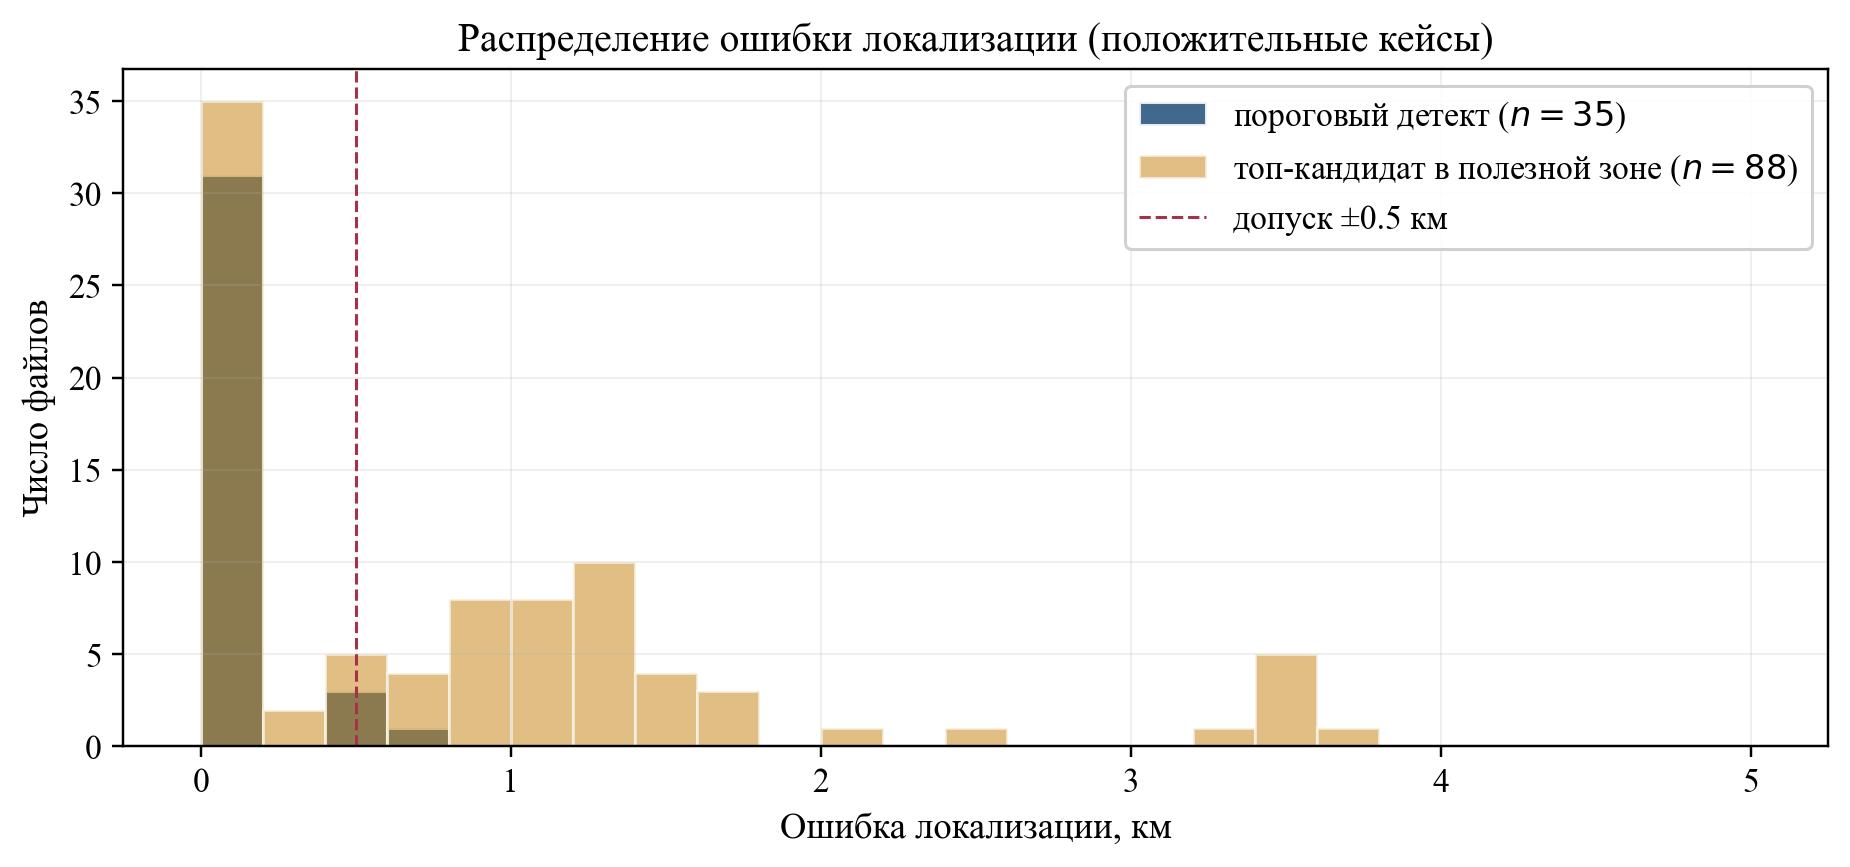
\includegraphics[width=0.95\textwidth]{fig_loc_err_hist.png}
  \caption{Распределение ошибки локализации на положительных кейсах. Тёмные столбцы - детекции, прошедшие двойной пороговый отбор; жёлтые - топ-кандидат в полезной зоне (включая случаи, где топ-кандидат лежит вне допуска).}
  \label{fig:loc_err_hist}
\end{figure}

Ту же информацию иллюстрирует диаграмма рассеяния «детектированная~- истинная позиция» (рис.~\ref{fig:scatter}): для попаданий точки лежат вблизи диагонали, тогда как промахи рассыпаны вертикально вдоль четырёх характерных значений истинной позиции (по числу размеченных линий и схем воздействия).

\begin{figure}[h]
  \centering
  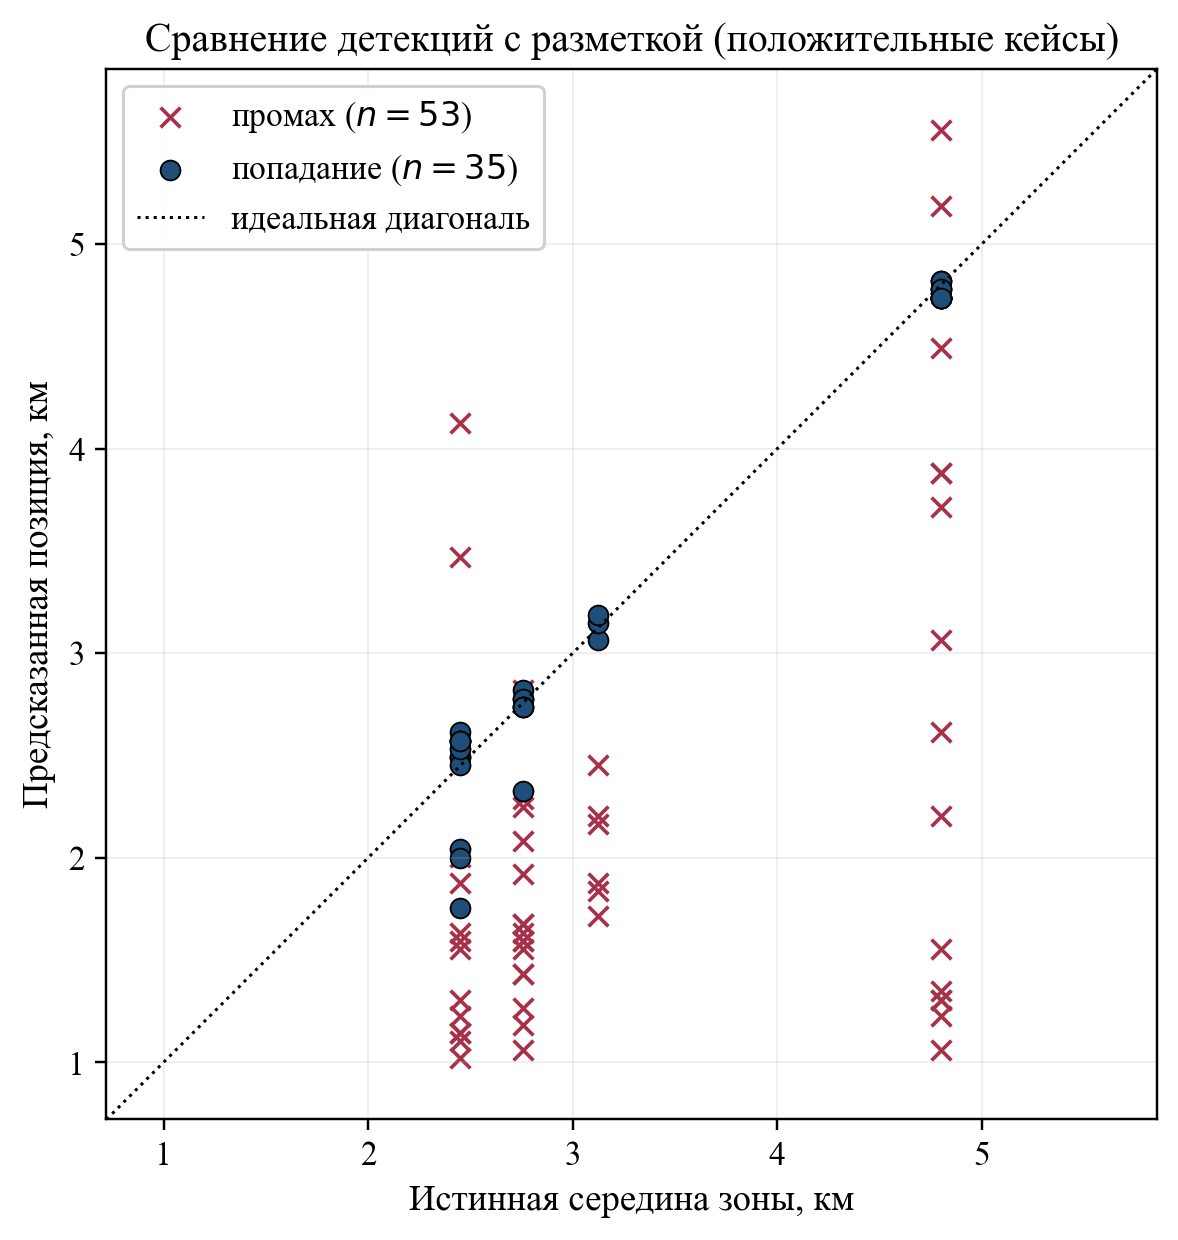
\includegraphics[width=0.62\textwidth]{fig_scatter.png}
  \caption{Сравнение детекций с разметкой на положительных кейсах. По горизонтали - середина эталонной зоны, по вертикали - позиция топ-кандидата в полезной зоне.}
  \label{fig:scatter}
\end{figure}

Recall заметно зависит от длительности зондирующего импульса (таблица~\ref{tab:pulse}, рис.~\ref{fig:recall_by_pulse}). Наилучший пороговый Recall достигается на средних длительностях 200-500~нс ($0{,}50$, $0{,}59$ и $0{,}55$). На 100~нс пороговый Recall падает до $0{,}11$, поскольку короткий импульс даёт меньшее SNR в каждом дистанционном бине и слабые воздействия не выходят за двойной пороговый отбор; в режиме топ-кандидата при той же выборке Recall составляет $0{,}28$ - значит, событие в наиболее аномальной группе обнаруживается чаще, чем порог пропускает. На 1000~нс пороговый Recall падает до $0{,}19$ из-за пространственного «размытия» воздействия: для длинного импульса событие распределяется на $\sim 100$~м, и пиковое значение оценки $S(g)$ в любом отдельно взятом дистанционном бине оказывается ниже. На 500~нс пороговый Recall ($0{,}55$) формально превышает Recall топ-кандидата ($0{,}50$) - такое возможно за счёт того, что пороговый режим может зафиксировать несколько кандидатов на одной записи и засчитать попадание любого из них, тогда как режим топ-кандидата берёт лишь одну группу с максимальным $S(g)$, и в нескольких файлах эта группа лежит вне эталонной зоны.

\begin{table}[h]
\caption{Recall по длительности зондирующего импульса.}
\label{tab:pulse}
\centering
\renewcommand{\arraystretch}{1.2}
\begin{tabular}{l r r r}
\toprule
\textbf{Импульс} & $n$ & \textbf{Recall (порог)} & \textbf{Recall (топ-кандидат)} \\
\midrule
100 нс & 18 & 0{,}11 (2/18) & 0{,}28 (5/18) \\
200 нс & 16 & 0{,}50 (8/16) & 0{,}69 (11/16) \\
300 нс & 17 & 0{,}59 (10/17) & 0{,}71 (12/17) \\
500 нс & 20 & 0{,}55 (11/20) & 0{,}50 (10/20) \\
1000 нс & 21 & 0{,}19 (4/21) & 0{,}24 (5/21) \\
\midrule
\textbf{Итого} & \textbf{92} & \textbf{0{,}38} (35/92) & \textbf{0{,}47} (43/92) \\
\bottomrule
\end{tabular}
\end{table}

\begin{figure}[h]
  \centering
  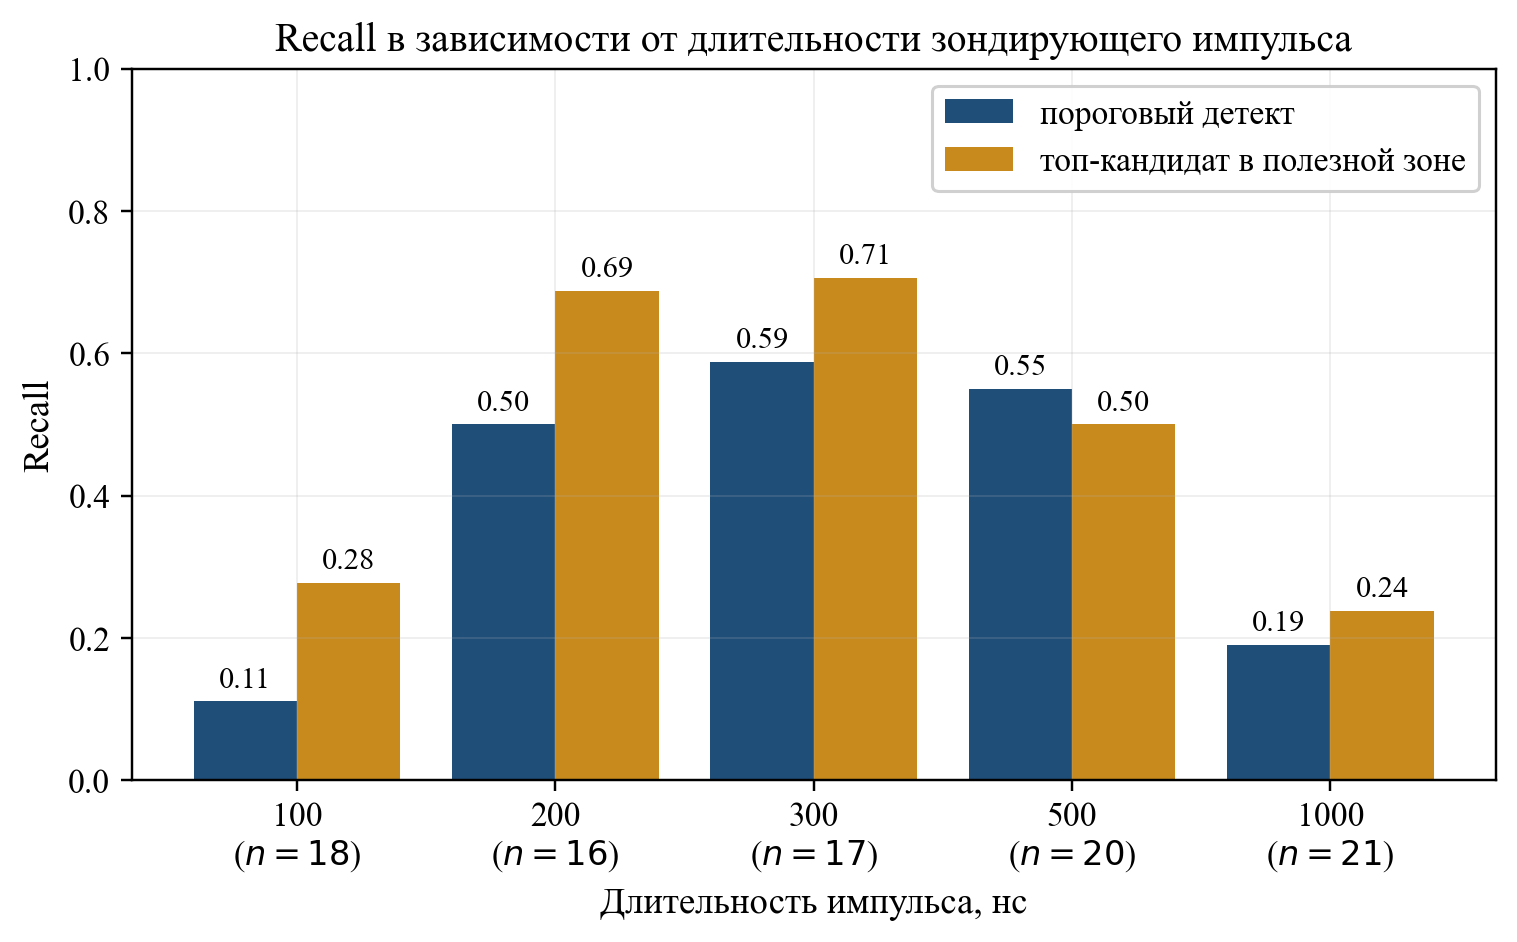
\includegraphics[width=0.85\textwidth]{fig_recall_by_pulse.png}
  \caption{Recall на положительных кейсах в зависимости от длительности зондирующего импульса.}
  \label{fig:recall_by_pulse}
\end{figure}

% ---- 4.4 Сравнение с детекторами-эталонами ----
\subsection{Сравнение с одно-компонентными детекторами-эталонами}
\label{sec:ablation}

Для обоснования выбора комбинированной оценки $S(g)$ (формула~\eqref{eq:combined}) проведено сравнение с тремя альтернативными вариантами при идентичном остальном алгоритме (парсер, выравнивание, шаги 1-4 детектора) и идентичной процедуре пороговой фильтрации, отличающейся только источником оценки. Рассматриваются:
\begin{itemize}[leftmargin=2em]
  \item \textbf{Комбинированный (ослабленный)} - комбинированная оценка с ослабленными порогами ($S_\text{thr} = \mathrm{med} + 2\,\mathrm{MAD}$, $P_\text{thr} = \mathrm{med} + 3\,\mathrm{MAD}$);
  \item \textbf{Только пик} - оценка равна только спектральному пику $\mathrm{peak}(g)$, одиночный порог на $3\,\sigma$;
  \item \textbf{Только энергия} - оценка равна только $\mathrm{energy\_z}(g)$, одиночный порог на $3\,\sigma$.
\end{itemize}
Результаты приведены в таблице~\ref{tab:ablation} и на рис.~\ref{fig:f1_bars}.

\begin{table}[h]
\caption{Сравнение детекторов на размеченном наборе из 130 файлов.}
\label{tab:ablation}
\centering
\renewcommand{\arraystretch}{1.2}
\begin{tabular}{l r r r r r}
\toprule
\textbf{Детектор} & \textbf{Recall} & \textbf{Precision} & \textbf{F1} & \textbf{FP} & \textbf{Ошибка лок., м} \\
\midrule
Комбинированный (предложенный) & 0{,}380 & \textbf{0{,}636} & \textbf{0{,}476} & 20 & 61 \\
Комбинированный (ослабленный) & 0{,}424 & 0{,}371 & 0{,}396 & 66 & 61 \\
Только пик & \textbf{0{,}478} & 0{,}383 & 0{,}425 & 71 & 61 \\
Только энергия & 0{,}391 & 0{,}288 & 0{,}332 & 89 & 61 \\
\bottomrule
\end{tabular}
\end{table}

\begin{figure}[h]
  \centering
  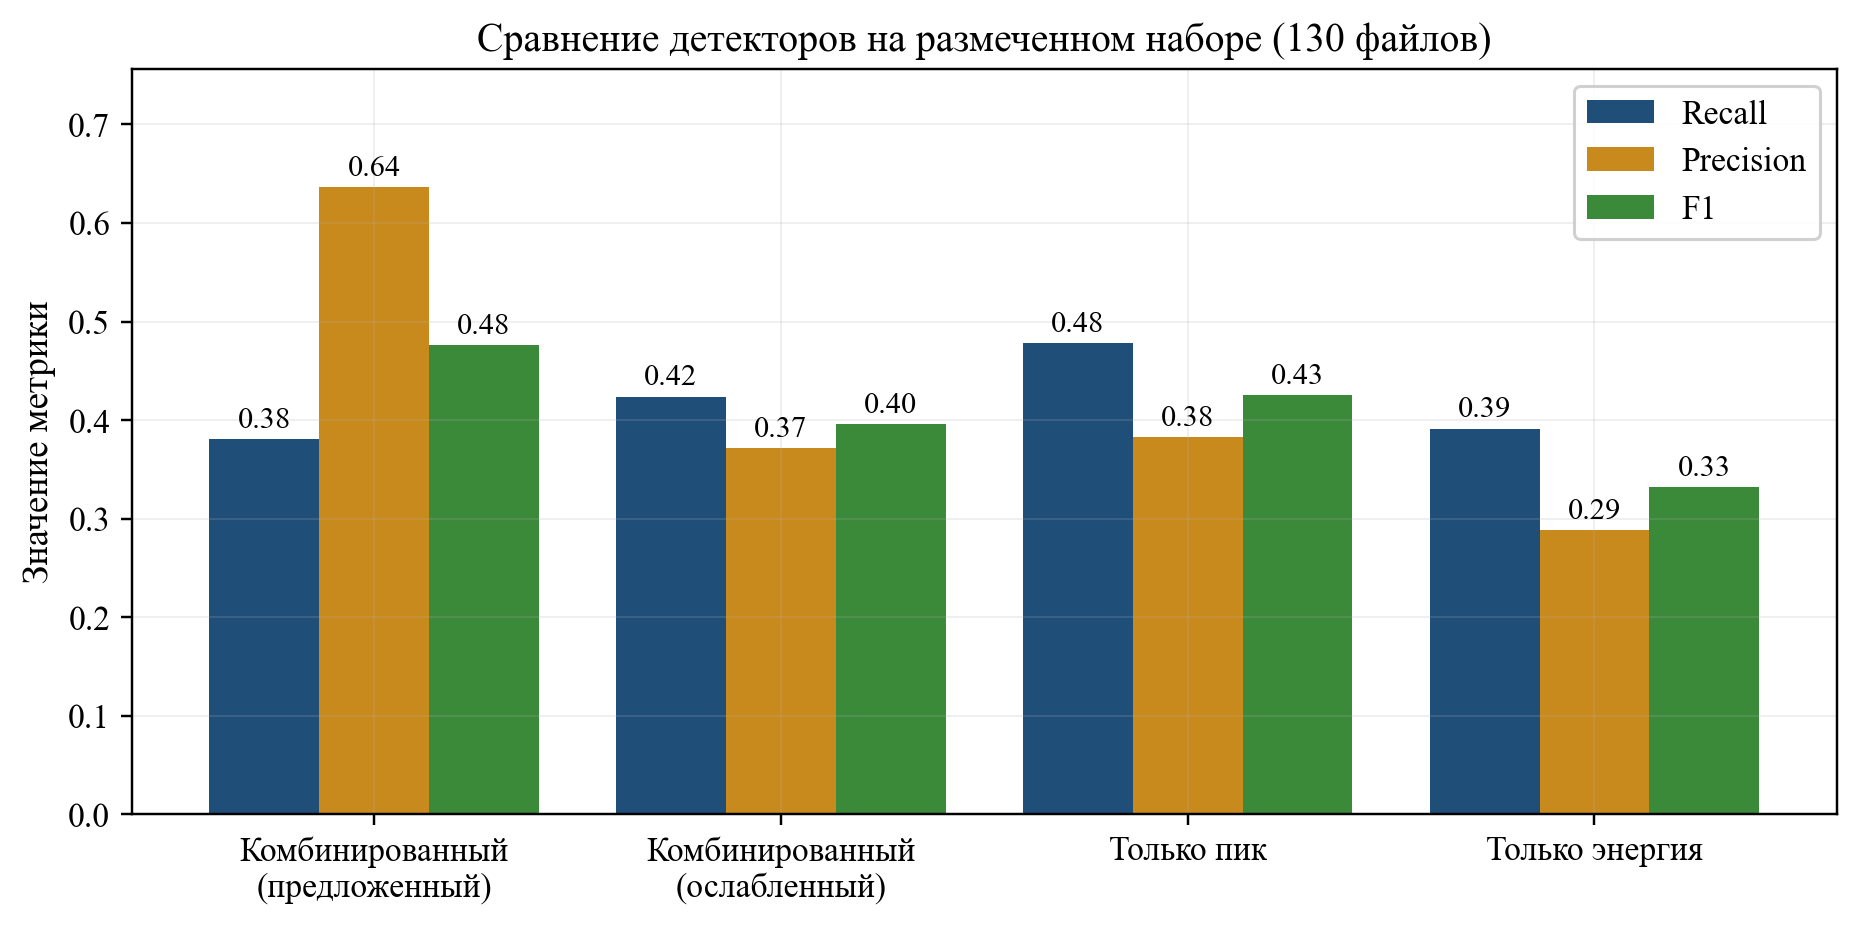
\includegraphics[width=0.95\textwidth]{fig_f1_bars.png}
  \caption{Recall, Precision и F1-мера четырёх детекторов на размеченном наборе.}
  \label{fig:f1_bars}
\end{figure}

\noindent
Выводы по сравнению:
\begin{enumerate}[leftmargin=2.5em, label=(\arabic*)]
  \item \textbf{Комбинированный детектор лидирует по F1-мере} ($0{,}476$ против $0{,}425$ у варианта «только пик» и $0{,}332$ у варианта «только энергия»). Это означает, что введение двойного порогового отбора и трёхкомпонентной оценки $S(g)$ улучшает соотношение Recall/Precision не менее чем на 5~абсолютных процентных пунктов.
  \item \textbf{Детектор «только энергия» - слабейший вариант} (F1 $= 0{,}33$). Энергетический детектор не различает локализованную аномалию и стационарно шумящий участок линии (например, вблизи усилителя), что даёт почти в 4{,}5 раза больше ложных срабатываний, чем комбинированный детектор. Этот результат непосредственно отвечает на вопрос «зачем не использовать простой энергетический детектор» - на длинной линии с усилителями он систематически тонет в неоднородности фона.
  \item \textbf{Детектор «только пик» достигает максимального Recall} ($0{,}478$), но платит за это Precision: половина детекций отнесена к точкам, не размеченным как события. Это ожидаемое поведение метода, который флагирует любой выраженный спектральный максимум без дополнительной проверки на стабильность пространственного пика.
  \item \textbf{Точность локализации совпадает} у всех четырёх вариантов - медиана 61~м. Различие между методами проявляется в том, \textit{какие} зоны они флагируют выше порога, а не в том, \textit{где именно} они фиксируют пик внутри уже выбранной зоны.
\end{enumerate}

% ---- 4.5 Ограничения метода ----
\subsection{Ограничения метода}
\label{sec:limitations}

Анализ результатов выявляет несколько принципиальных ограничений, не устранимых в рамках существующего алгоритма без его существенной модификации.

\textbf{Плато Recall на уровне $\sim 0{,}47$.} Максимальное значение Recall в режиме топ-кандидата составляет $0{,}467$ и не зависит от ослабления порогов; это означает, что приблизительно для половины положительных кейсов наиболее спектрально аномальная группа в полезной зоне не попадает в эталонную зону вообще. Анализ этих файлов показывает, что во многих из них частота воздействия (например, шаги человека по грунту с темпом $\approx 0{,}57$~Гц) лежит ниже частотного разрешения окна записи: при длительности 1~с и темпе одного полного цикла $\approx 1{,}75$~с спектральная составляющая шага попадает в первую частотную ячейку $f \in [0, 1]$~Гц, отсечённую границей $f_\text{min} = 5$~Гц. Детектор полагается на широкополосные импактные составляющие (5-100~Гц), которые слабее самого периодического воздействия и не всегда устойчиво превышают шум линии.

\textbf{Длительные тестовые записи: пустой пороговый детект.} На непрерывных записях длительностью около 10~секунд фон линии заметно дрейфует во времени; стационарная модель «медианно-MAD по времени» перестаёт быть адекватной. Эта проблема устранима введением скользящей по времени нормировки сегментами длительностью около 1~секунды, что относится к задачам дальнейшего исследования.

\textbf{Зависимость от длительности импульса.} На 100~нс импульсах Recall падает из-за низкого SNR одиночного отсчёта; на 1000~нс - из-за пространственного размытия события на $\sim 100$~м, превышающего размер пространственной группы $G \cdot \Delta x = 20 \cdot 2$~м. Возможное направление улучшения - адаптивный выбор $G$ под конкретное пространственное разрешение установки.

\textbf{Ограниченность отрицательного набора.} Все 38 размеченных отрицательных кейсов получены на одной из четырёх оптических линий установки и одной длительности зондирующего импульса (500~нс). Полученное значение Precision $= 0{,}636$ следует трактовать как оценку сверху - на репрезентативном наборе отрицательных кейсов с разных линий и при разных длительностях импульса Precision, по-видимому, окажется ниже. Расширение размеченного набора отрицательных примеров - отдельная задача дальнейшей работы.

\newpage

% =====================================================================
%  5. ЗАКЛЮЧЕНИЕ
% =====================================================================
\section{Заключение}

В рамках работы разработан и валидирован воспроизводимый алгоритм обработки данных фазочувствительной оптической рефлектометрии на длинных оптических линиях с распределёнными EDFA-усилителями. Проведённый анализ существующих подходов к локализации возмущений в \phiOTDR{} - на основе непрерывного вейвлет-преобразования~\cite{Qin2012}, преобразования Гильберта–Хуанга~\cite{Hui2014}, разложения по вейвлет-пакетам~\cite{Li2014}, сравнения матриц расстояний между трассами~\cite{Liu2018}, а также методов машинного обучения~\cite{Wu2019, Shi2020} - показал, что существующие методы либо ориентированы на короткие линии и не учитывают неоднородность фона при наличии распределённых усилителей, либо выдают результат в виде двумерной карты в плоскости (частота, дистанция), требующей дополнительной интерпретации, либо требуют размеченных наборов данных в объёмах, нехарактерных для лабораторных установок. Этот пробел определил структуру разрабатываемого метода.

Реализован полный алгоритм обработки. На вход подаётся непрерывная запись аналого-цифрового преобразователя; парсер с автооценкой периода следования зондирующих импульсов выделяет из неё отдельные рефлектограммы - на полном наборе из 552 непрерывных записей корректно обработаны 535 (96{,}9~\%) с медианным коэффициентом покрытия, равным единице. Далее выполняется кросс-корреляционное межтрассовое выравнивание с тремя критериями приёма (по средней невязке, по 95-му перцентилю и по межтрассовой шероховатости); на основной массе записей медианная невязка после выравнивания близка к нулю. Финальный этап - устойчивый к выбросам детектор возмущений, последовательно выполняющий вычитание медианного фона по времени, MAD-нормировку остатка по дистанционным бинам, группировку и преобразование Фурье по времени, устойчивую к выбросам нормировку спектра по частоте и скаляризацию в одномерную комбинированную оценку $S(g) = 0{,}55\cdot\mathrm{peak} + 0{,}30\cdot\mathrm{broad} + 0{,}15\cdot\mathrm{energy\_z}$ с двойным пороговым отбором кандидатов и подавлением повторов на масштабе 2~км.

Метод количественно валидирован на размеченном наборе из 130 записей (92 положительных и 38 отрицательных кейсов). При едином наборе гиперпараметров достигнуты F1-мера 0{,}48 при Precision 0{,}64 и Recall 0{,}38; медианная ошибка локализации составляет 61~м, что для эталонной размеченной зоны даёт относительную ошибку около $1\,\%$. Сравнение с одно-компонентными детекторами-эталонами при идентичном остальном алгоритме показывает, что замена комбинированной оценки $S(g)$ на любую из трёх компонент существенно ухудшает F1-меру: 0{,}43 для одного спектрального пика и 0{,}33 для энергетического детектора. Этот результат прямо отвечает на основной методический вопрос - объединение спектральных признаков с устойчивой к выбросам MAD-нормировкой по дистанции даёт качественный прирост точности по сравнению с простыми энергетическими методами в условиях неоднородного по дистанции фона длинной линии с распределёнными усилителями.

Практическая значимость работы состоит в том, что предложенный метод сворачивает двумерное представление сигнала в плоскости (частота, дистанция) в одномерную оценку $S(g)$ по дистанции, что упрощает интерпретацию и хранение результата по сравнению с двумерными тепловыми картами, типичными для методов на основе вейвлет-разложения. Двойной пороговый отбор подавляет ложные срабатывания, характерные для энергетических детекторов в зонах с повышенным фоном вблизи усилителей. Метод не требует априорного знания спектральных характеристик возмущения и применим к данным \phiOTDR{} на длинных оптических линиях с EDFA-усилением; при этом нечувствительность к медленным диффузным изменениям фона обеспечивает устойчивость детектора к естественным фоновым процессам - суточному ходу температуры, дрейфу мощности лазера, изменению усиления в EDFA - и потенциально снижает уровень ложных срабатываний, обусловленных такими процессами, в режиме длительного мониторинга. Количественная оценка Precision в эксплуатационных условиях требует отдельной валидации на расширенном отрицательном наборе с разных линий и при разных длительностях зондирующего импульса (см. раздел~\ref{sec:limitations}); полученное в работе значение Precision $= 0{,}64$ следует трактовать как оценку сверху для текущего размеченного набора. Отдельно отметим, что метод корректно отрабатывает уже на окне порядка $10^2$ рефлектограмм (около 0{,}1~секунды непрерывной записи на характерном для установки темпе следования зондирующих импульсов) и не требует дополнительной эталонной записи «спокойного» состояния линии - что выгодно отличает его от подходов на основе непрерывного вейвлет-преобразования и сопоставления матриц данных, требующих заметно более длинных окон или эталонного состояния.

В качестве направлений дальнейших исследований естественно выделить несколько задач, лежащих за пределами проектной области текущей реализации. Во-первых, введение скользящей по времени нормировки фона на сегментах длительностью около 1~секунды с последующей агрегацией оценки $S(g)$ между сегментами должно устранить деградацию детектора на длительных записях, где стационарная медианно-MAD модель перестаёт быть адекватной из-за дрейфа фона. Во-вторых, адаптивный выбор размера пространственной группы $G$ под конкретное пространственное разрешение установки позволит улучшить чувствительность к длинным зондирующим импульсам, на которых событие пространственно «размывается» за пределы фиксированной группы $G = 20$. В-третьих, существенно расширение валидационного набора в части отрицательных кейсов - текущая оценка Precision получена на одной из четырёх оптических линий и одной длительности зондирующего импульса и должна рассматриваться как оценка сверху. Наконец, учёт спектрального содержания ниже 5~Гц через переход к окну регистрации продолжительностью более 10~секунд может повысить Recall на медленных периодических воздействиях, ограниченных в текущей реализации нижней частотной отсечкой $f_\text{min} = 5$~Гц.

\newpage

% =====================================================================
%  СПИСОК ИСПОЛЬЗОВАННЫХ ИСТОЧНИКОВ
% =====================================================================
\renewcommand{\refname}{\hfill Список использованных источников \hfill}

\begin{thebibliography}{99}
  \fontsize{12}{14}\selectfont

  \bibitem{Lu2019}
  Lu,~P. Distributed optical fiber sensing: Review and perspective / P.~Lu, N.~Lalam, M.~Badar, B.~Liu, B.~T.~Chorpening, M.~P.~Buric, P.~R.~Ohodnicki // Applied Physics Reviews.~- 2019.~- Vol.~6, no.~4.~- P.~041302.~- doi: 10.1063/1.5113955.

  \bibitem{Palmieri2013}
  Palmieri,~L. Distributed Optical Fiber Sensing Based on Rayleigh Scattering / L.~Palmieri, L.~Schenato // The Open Optics Journal.~- 2013.~- Vol.~7.~- P.~104-127.~- doi: 10.2174/1874328501307010104.

  \bibitem{Bao2012}
  Bao,~X. Recent Progress in Distributed Fiber Optic Sensors / X.~Bao, L.~Chen // Sensors.~- 2012.~- Vol.~12, no.~7.~- P.~8601-8639.~- doi: 10.3390/s120708601.

  \bibitem{He2021}
  He,~Z. Optical Fiber Distributed Acoustic Sensors: A Review / Z.~He, Q.~Liu // Journal of Lightwave Technology.~- 2021.~- Vol.~39, no.~12.~- P.~3671-3686.~- doi: 10.1109/JLT.2021.3059771.

  \bibitem{Muanenda2018}
  Muanenda,~Y. Recent Advances in Distributed Acoustic Sensing Based on Phase-Sensitive Optical Time Domain Reflectometry / Y.~Muanenda // Journal of Sensors.~- 2018.~- Vol.~2018.~- Article ID~3897873.~- 16~p.~- doi: 10.1155/2018/3897873.

  \bibitem{Posey2000}
  Posey,~R., Jr. Strain sensing based on coherent Rayleigh scattering in an optical fibre / R.~Posey, Jr., G.~A.~Johnson, S.~T.~Vohra // Electronics Letters.~- 2000.~- Vol.~36, no.~20.~- P.~1688-1689.~- doi: 10.1049/el:20001200.

  \bibitem{Juarez2005}
  Juarez,~J.~C. Distributed fiber-optic intrusion sensor system / J.~C.~Juarez, E.~W.~Maier, K.~N.~Choi, H.~F.~Taylor // Journal of Lightwave Technology.~- 2005.~- Vol.~23, no.~6.~- P.~2081-2087.~- doi: 10.1109/JLT.2005.849924.

  \bibitem{Lu2010}
  Lu,~Y. Distributed Vibration Sensor Based on Coherent Detection of Phase-OTDR / Y.~Lu, T.~Zhu, L.~Chen, X.~Bao // Journal of Lightwave Technology.~- 2010.~- Vol.~28, no.~22.~- P.~3243-3249.~- doi: 10.1109/JLT.2010.2078798.

  \bibitem{Wang2016}
  Wang,~Z. Coherent $\Phi$-OTDR based on I/Q demodulation and homodyne detection / Z.~Wang, L.~Zhang, S.~Wang, N.~Xue, F.~Peng, M.~Fan, W.~Sun, X.~Qian, J.~Rao, Y.~Rao // Optics Express.~- 2016.~- Vol.~24, no.~2.~- P.~853-858.~- doi: 10.1364/OE.24.000853.

  \bibitem{PastorGraells2016}
  Pastor-Graells,~J. Single-shot distributed temperature and strain tracking using direct detection phase-sensitive OTDR with chirped pulses / J.~Pastor-Graells, H.~F.~Martins, A.~Garcia-Ruiz, S.~Martin-Lopez, M.~Gonzalez-Herraez // Optics Express.~- 2016.~- Vol.~24, no.~12.~- P.~13121-13133.~- doi: 10.1364/OE.24.013121.

  \bibitem{Pang2016}
  Pang,~F. A Fading-Discrimination Method for Distributed Vibration Sensor Using Coherent Detection of $\Phi$-OTDR / F.~Pang, M.~He, H.~Liu, X.~Mei, J.~Tao, T.~Zhang, X.~Zhang, N.~Chen, T.~Wang // IEEE Photonics Technology Letters.~- 2016.~- Vol.~28, no.~23.~- P.~2752-2755.~- doi: 10.1109/LPT.2016.2616023.

  \bibitem{Peng2014}
  Peng,~F. Ultra-long high-sensitivity $\Phi$-OTDR for high spatial resolution intrusion detection of pipelines / F.~Peng, H.~Wu, X.-H.~Jia, Y.-J.~Rao, Z.-N.~Wang, Z.-P.~Peng // Optics Express.~- 2014.~- Vol.~22, no.~11.~- P.~13804-13810.~- doi: 10.1364/OE.22.013804.

  \bibitem{WangZN2014}
  Wang,~Z.~N. Ultra-long phase-sensitive OTDR with hybrid distributed amplification / Z.~N.~Wang, J.~J.~Zeng, J.~Li, M.~Q.~Fan, H.~Wu, F.~Peng, L.~Zhang, Y.~Zhou, Y.~J.~Rao // Optics Letters.~- 2014.~- Vol.~39, no.~20.~- P.~5866-5869.~- doi: 10.1364/OL.39.005866.

  \bibitem{Martins2014}
  Martins,~H.~F. Phase-sensitive Optical Time Domain Reflectometer Assisted by First-order Raman Amplification for Distributed Vibration Sensing Over $>$100~km / H.~F.~Martins, S.~Martin-Lopez, P.~Corredera, M.~L.~Filograno, O.~Frazão, M.~Gonzalez-Herraez // Journal of Lightwave Technology.~- 2014.~- Vol.~32, no.~8.~- P.~1510-1518.~- doi: 10.1109/JLT.2014.2308354.

  \bibitem{Tian2016}
  Tian,~X.~Z. 123 km $\Phi$-OTDR system based on bidirectional erbium-doped fiber amplifier / X.~Z.~Tian, R.~Dang, D.~J.~Tan, L.~Liu, H.~M.~Wang // Proc. SPIE.~- 2016.~- Vol.~10158: Optical Communication, Optical Fiber Sensors, and Optical Memories for Big Data Storage.~- P.~101580P.~- doi: 10.1117/12.2246763.

  \bibitem{Wang2023}
  Wang,~Y. 190~km $\Phi$-OTDR with bidirectional Raman and relay erbium-doped fiber hybrid amplification / Y.~Wang, Y.~Wang, C.~He, X.~Liu, Q.~Bai, B.~Jin // Optics and Lasers in Engineering.~- 2023.~- Vol.~166.~- P.~107569.~- doi: 10.1016/j.optlaseng.2023.107569.

  \bibitem{Fan2023}
  Fan,~C. 300 km ultralong fiber optic DAS system based on optimally designed bidirectional EDFA relays / C.~Fan, H.~Li, K.~Zhang, H.~Liu, Y.~Sun, H.~Liu, B.~Yan, Z.~Yan, D.~Liu, P.~P.~Shum, Q.~Sun // Photonics Research.~- 2023.~- Vol.~11, no.~6.~- P.~968-977.~- doi: 10.1364/PRJ.485701.

  \bibitem{Qin2012}
  Qin,~Z. Continuous wavelet transform for non-stationary vibration detection with phase-OTDR / Z.~Qin, L.~Chen, X.~Bao // Optics Express.~- 2012.~- Vol.~20, no.~18.~- P.~20459-20465.~- doi: 10.1364/OE.20.020459.

  \bibitem{Hui2014}
  Hui,~X. Hilbert–Huang Transform Time-Frequency Analysis in $\Phi$-OTDR Distributed Sensor / X.~Hui, S.~Zheng, J.~Zhou, H.~Chi, X.~Jin, X.~Zhang // IEEE Photonics Technology Letters.~- 2014.~- Vol.~26, no.~23.~- P.~2403-2406.~- doi: 10.1109/LPT.2014.2358262.

  \bibitem{Li2014}
  Li,~Q. Fiber-optic distributed sensor based on phase-sensitive OTDR and wavelet packet transform for multiple disturbances location / Q.~Li, C.~Zhang, C.~Li // Optik.~- 2014.~- Vol.~125, no.~24.~- P.~7235-7238.~- doi: 10.1016/j.ijleo.2014.07.128.

  \bibitem{Liu2018}
  Liu,~X. Real-Time Phase-Sensitive OTDR Based on Data Matrix Matching Method / X.~Liu, Y.~Wang, R.~Wu, D.~Wang, Q.~Bai, B.~Jin // Sensors.~- 2018.~- Vol.~18, no.~6.~- P.~1883.~- doi: 10.3390/s18061883.

  \bibitem{Tejedor2017}
  Tejedor,~J. A Novel Fiber Optic Based Surveillance System for Prevention of Pipeline Integrity Threats / J.~Tejedor, J.~Macias-Guarasa, H.~F.~Martins, D.~Piote, J.~Pastor-Graells, S.~Martin-Lopez, P.~Corredera, M.~Gonzalez-Herraez // Sensors.~- 2017.~- Vol.~17, no.~2.~- P.~355.~- doi: 10.3390/s17020355.

  \bibitem{Wu2019}
  Wu,~H. A Dynamic Time Sequence Recognition and Knowledge Mining Method Based on the Hidden Markov Models (HMMs) for Pipeline Safety Monitoring With $\Phi$-OTDR / H.~Wu, X.~Liu, Y.~Xiao, Y.~Rao // Journal of Lightwave Technology.~- 2019.~- Vol.~37, no.~19.~- P.~4991-5000.~- doi: 10.1109/JLT.2019.2926745.

  \bibitem{Shi2020}
  Shi,~Y. Multi-event classification for $\Phi$-OTDR distributed optical fiber sensing system using deep learning and support vector machine / Y.~Shi, Y.~Wang, L.~Wang, L.~Zhao, Z.~Fan // Optik.~- 2020.~- Vol.~221.~- P.~165373.~- doi: 10.1016/j.ijleo.2020.165373.

  \bibitem{Hampel1974}
  Hampel,~F.~R. The Influence Curve and its Role in Robust Estimation / F.~R.~Hampel // Journal of the American Statistical Association.~- 1974.~- Vol.~69, no.~346.~- P.~383-393.~- doi: 10.1080/01621459.1974.10482962.

\end{thebibliography}

\end{document}
